%% -----------------------------------------------------------------------------

\chapter{Evaluation}\label{ch:evaluation}
\glsresetall % Resets all acronyms to not used

In this chapter, the proposed technique for detecting sender MAC addresses during collisions is evaluated using several simulations as well as experiments on WARP software-defined radios.

Possible questions and problems include the fact, that with higher \glspl{MCS}, there could be not enough samples to correlate the rather short 6 byte MAC address. Another interesting issue is the accuracy of the algorithm with increasing amounts of noise and fading.


%% -----------------------------------------------------------------------------

\section{Frequency-Domain Correlation}\label{sec:freqd-correlation}

During the implementation of the MAC address detection technique, I tried using cross-correlation in the frequency-domain. This means that instead of calculating the similarity between samples, complex symbols are correlated without mapping them into the time-domain. With this approach, the Fourier transform must be applied to the received signal.

It turns out to be at least very difficult, if not impossible, to detect senders in case of a collision with frequency-domain correlation. The reason for that is phase shift due to path delays. When a signal is received with an offset in the time-domain, the constellation is changed in the frequency-domain. This can be shown using the Fourier transform equation:

$$ F(f) = \int_{-\infty}^{\infty} s(t) \cdot e^{-2 \pi i f t} dt $$\vspace{0cm}

Here, $ i $ is the imaginary unit, $ F(f) $ is the Fourier transform at frequency $ f $, and $ s(t) $ is the time-domain signal depending on $ t $. A time offset can now be expressed as $ t + \Delta $. Standard power laws then show that this offset introduces a constant multiplication factor on $ F(f) $, depending on $ \Delta $.

$$ F(f) = \int_{-\infty}^{\infty} s(t + \Delta) \cdot e^{-2 \pi i f \cdot (t + \Delta)} dt = \int_{-\infty}^{\infty} s(t + \Delta) \cdot e^{-2 \pi i f t} \cdot e^{-2 \pi i f \Delta} dt = $$
$$ = e^{-2 \pi i f \Delta} \cdot \int_{-\infty}^{\infty} s(t + \Delta) \cdot e^{-2 \pi i f t} dt $$\vspace{0cm}

Since both $ s(t) $ and $ F(f) $ are complex functions, this multiplication is a rotation, or phase shift, in the complex constellation plane. Furthermore, the rotation is different for different frequencies $ f $.

This leads to a received constellation similar to that shown in figure \ref{fig:freqd-corr}. To create this figure, I applied a Rayleigh channel \cite{NEEDED} to a simulated collision signal, introducing a delay of a few nanoseconds. The signals are modulated with BPSK, so ideally the only constellation points should be $ 1 $ and $ -1 $. However, due to the above described rotation, the constellation is basically a circle.

\begin{figure}[ht]
	\centering
	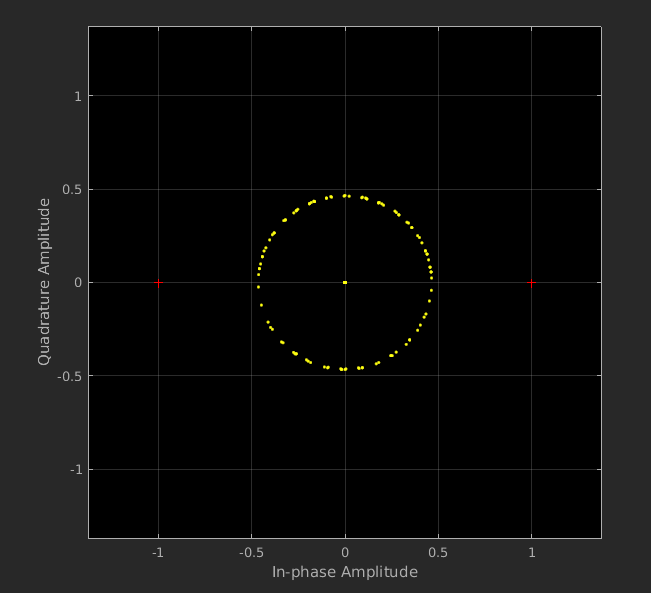
\includegraphics[width=8cm]{gfx/images/freqd-correlation}
	\caption{Cross Correlation of Frequency-Domain Symbols after Channel}
	\label{fig:freqd-corr}
\end{figure}

This kind of path effects is not at all unusual in a IEEE 802.11 transmission. Under normal circumstances, the known preamble is used to calculate the inverted channel matrix of the path effects, as mentioned in section \ref{sec:multipath}.

When receiving a collision, there is however not only one preamble. Instead, the preambles of two different frames, which experienced different path effects, are added together. Since the preambles itself are designed to have a low autocorrelation \cite{NEEDED}, it is not easily possible to separate the two channel effects from each other. Therefore, I can not reverse the phase shift introduced on the OFDM symbols containing the MAC address.

As expected, experiments with cross-correlation in the frequency-domain without channel equalization were unsuccessful. I therefore disregarded this approach.


%% -----------------------------------------------------------------------------

\section{Time-Domain Correlation}

The experiments I did using time-domain cross-correlation are devided in two groups. First, I used Matlab to simulate different field variations and channel effects. Second, I used WARP boards to try the approach in a real-world scenario. The results of these experiments are summarized in the following sections.

When correlating time-domain samples, I always pre-generated reference samples and calculated the correlation only for the subset of samples that contains the MAC address. Section \ref{sec:mac-periods} describes which period of the signal this is.\\

Reference signals are modulated until just after the Fourier transform and adding of cyclic prefix. For the simulations, I used a sampling rate of 20 MHz, which is the default output of the Matlab WLAN System Toolbox. The WARP boards use a sampling frequency of 40 MHz however, so for these experiments I used interpolation to double the rate.

All experiments used realistic real-world MAC addresses, as described in section \ref{sec:real-world-macs}.


%% -----------------------------------------------------------------------------

\section{Real-World MAC Addresses}\label{sec:real-world-macs}

MAC addresses are 6 byte numbers, where the first 3 bytes are a vendor prefix, identifying the company that built the network interface. The remaining 3 bytes are a unique identifier for the specific hardware.

After initial tries with some artificial MAC addresses in the form of AB:CD:EF:12:34:56, I switched to using a sample set of real-world MAC addresses. This allowed for a closer simulation of an actual use-case for sender detection.\\

I collected 64 MAC addresses from devices that were connected to the wireless university eduroam network. The gathering was done in the afternoon on a weekday. I used airodump from the \texttt{aircrack-ng} software suite to dump all MAC addresses on the network into a file. The actual command looked like this:

\begin{lstlisting}[captionpos=b,caption={Capture Real-World MAC Addresses},label=lst:airodump]
airmon-ng start wlp0s20u1
airodump-ng --essid eduroam -a -o csv -w mac-addresses-eduroam.csv wlp0s20u1mon
\end{lstlisting}

It is important to have the wireless network interface set to promiscuitive mode. This mode instructs the driver to hand all received frames to the kernel. Otherwise, only frames that are addressed to or coming from the local station are gathered, while the rest is filtered. This would mean that only the router's and the station's own MAC address would be cached.

In a possible real-time usage scenario of the sender detection algorithm, it would also be important to use promiscuous mode in order to collect all MAC addresses. These are the addresses for which reference signals need to be modulated and cached.


%% -----------------------------------------------------------------------------

\section{Modulation and Coding Schemes}

Intuitively, the overall sender detection accuracy should decrease for higher \glspl{MCS}. Firstly, with a higher \gls{MCS} there are more payload bits encoded in every \gls{OFDM} symbol, as described in table \ref{tbl:mcs}. This means that when applying cross-correlation, the \gls{OFDM} symbol contains random data from the MAC header before and after the sender MAC address. Due to the nature of \gls{OFDM}, it is not possible to limit correlation to only a fraction of the symbol in the time-domain.

Secondly, the higher constellation itself, which comes with higher \gls{MCS}, means that payload data gets mapped to complex points in the constellation plane that are less distinct from each other. Therefore, different data can seem more similar under cross-correlation, making it harder to detect senders in the time-domain.\\

To evaluate the detection algorithm's performance, I measured the correctness of detected MAC addresses for each of the 8 available \glspl{MCS}. For every \gls{MCS}, 1000 experiments were conducted. The results are the stacked sums of times where a completely correct pair of senders were guessed, times where only one of the senders was correct, and the amount of failures, in the sense of both addresses being incorrect.

Figure \ref{fig:vary_mcs} is the resulting plot. Different \glspl{MCS} are spread out on the x axis. The stacked bars show the amount of experiments for each result category as described above. As expected, the detection accuracy decreases for higher \glspl{MCS}. It is worth mentioning that for low \glspl{MCS}, the performance is very good, better than I expected. Furthermore, it seems to decrease exponentionally, but to justify this more data would be needed.

\begin{figure}[H]
	\centering
	\setlength\figureheight{5cm}
	\setlength\figurewidth{0.9\textwidth}
	% uncomment the following line to recompile the figure when it changes otherwise a cached version is used
	%\tikzset{external/remake next}
	% This file was created by matlab2tikz.
%
%The latest updates can be retrieved from
%  http://www.mathworks.com/matlabcentral/fileexchange/22022-matlab2tikz-matlab2tikz
%where you can also make suggestions and rate matlab2tikz.
%
\definecolor{mycolor1}{rgb}{0.24220,0.15040,0.66030}%
\definecolor{mycolor2}{rgb}{0.09640,0.75000,0.71204}%
\definecolor{mycolor3}{rgb}{0.97690,0.98390,0.08050}%
%
\begin{tikzpicture}[%
font=\footnotesize
]

\begin{axis}[%
width=0.951\figurewidth,
height=\figureheight,
at={(0\figurewidth,0\figureheight)},
scale only axis,
bar width=0.8,
xmin=0,
xmax=9,
xtick={1, 2, 3, 4, 5, 6, 7, 8},
xlabel style={font=\color{white!15!black}},
xlabel={MCS},
ymin=0,
ymax=1000,
ylabel style={font=\color{white!15!black}},
ylabel={\# experiments},
axis background/.style={fill=white},
title style={font=\bfseries},
title={Correct guesses for varying MCS},
legend style={at={(0.03,0.97)}, anchor=north west, legend cell align=left, align=left, draw=white!15!black},
clip mode=individual,transpose legend,legend columns=2,legend style={at={(0,1)},anchor=north west,draw=black,fill=white,legend cell align=left}
]
\addplot[ybar stacked, fill=mycolor1, draw=black, area legend] table[row sep=crcr] {%
1	0\\
2	0\\
3	0\\
4	0\\
5	8\\
6	0\\
7	75\\
8	296\\
};
\addplot[forget plot, color=white!15!black] table[row sep=crcr] {%
0	0\\
9	0\\
};
\addlegendentry{0 correct}

\addplot[ybar stacked, fill=mycolor2, draw=black, area legend] table[row sep=crcr] {%
1	0\\
2	0\\
3	1\\
4	0\\
5	95\\
6	118\\
7	481\\
8	527\\
};
\addplot[forget plot, color=white!15!black] table[row sep=crcr] {%
0	0\\
9	0\\
};
\addlegendentry{1 correct}

\addplot[ybar stacked, fill=mycolor3, draw=black, area legend] table[row sep=crcr] {%
1	1000\\
2	1000\\
3	999\\
4	1000\\
5	897\\
6	882\\
7	444\\
8	177\\
};
\addplot[forget plot, color=white!15!black] table[row sep=crcr] {%
0	0\\
9	0\\
};
\addlegendentry{2 correct}

\end{axis}
\end{tikzpicture}%
	\caption{Results: Varying MCS for 1000 experiments}
	\label{fig:vary_mcs}
\end{figure}


%% -----------------------------------------------------------------------------

\section{Scrambler initialization}\label{sec:ex-scrambler}

As described in section \ref{sec:mac-and-phy}, the MAC layer payload data is scrambled before any modulation on the physical layer is applied. The scrambling uses a 7 bit state register, where 0 is no valid state. Therefore, 127 unique scrambler initialization values are possible.

If the scrambler initialization is important for the sender detection technique, specifically if the modulated reference signals must use the same initialization as the received frames, the amount of possible values linearly scales the algorithm's complexity. That is, for every cached MAC address, \gls{MCS} et cetera all scrambler initializations must be modulated and correlated. It is therefore very interesting to know whether that is the case, or whether the scrambler alternatively does not affect detection quality.\\

Figure \ref{fig:vary_scrambler} shows the detection performance for different scrambler initializations over 1000 experiments. The data is presented the same way as in the previous section as stacked bar plots denoting the amount of runs with 0, 1, and 2 corrects guesses. For all experiments, the \gls{MCS} 0 was used. While the simulated received frame was modulated with scrambler initialization 1, correlation was calculated against 127 reference signals with different scrambler values.

The results show that indeed the scrambler initialization is very important for detection quality. While the performance is very good for the correct initialization value 1, for all other values the accuracy is low. However, related research mentions that some network interfaces seem to not choose the scrambler initialization at random \cite{NEEDED}, contradictory to the IEEE 802.11 standard. These devices use a static initialization for every frame, or increment the value after every transmission. This could be exploited by limiting the reference signals to such that are expected in the current network, therefore avoiding time spent on correlations that are unpromising. Since the MAC addresses of stations in the network are cached, the interface types and vendors are known. This could lead to some interesting future work.

\begin{figure}[H]
	\centering
	% uncomment the following line to recompile the figure when it changes otherwise a cached version is used
	%\tikzset{external/remake next}
	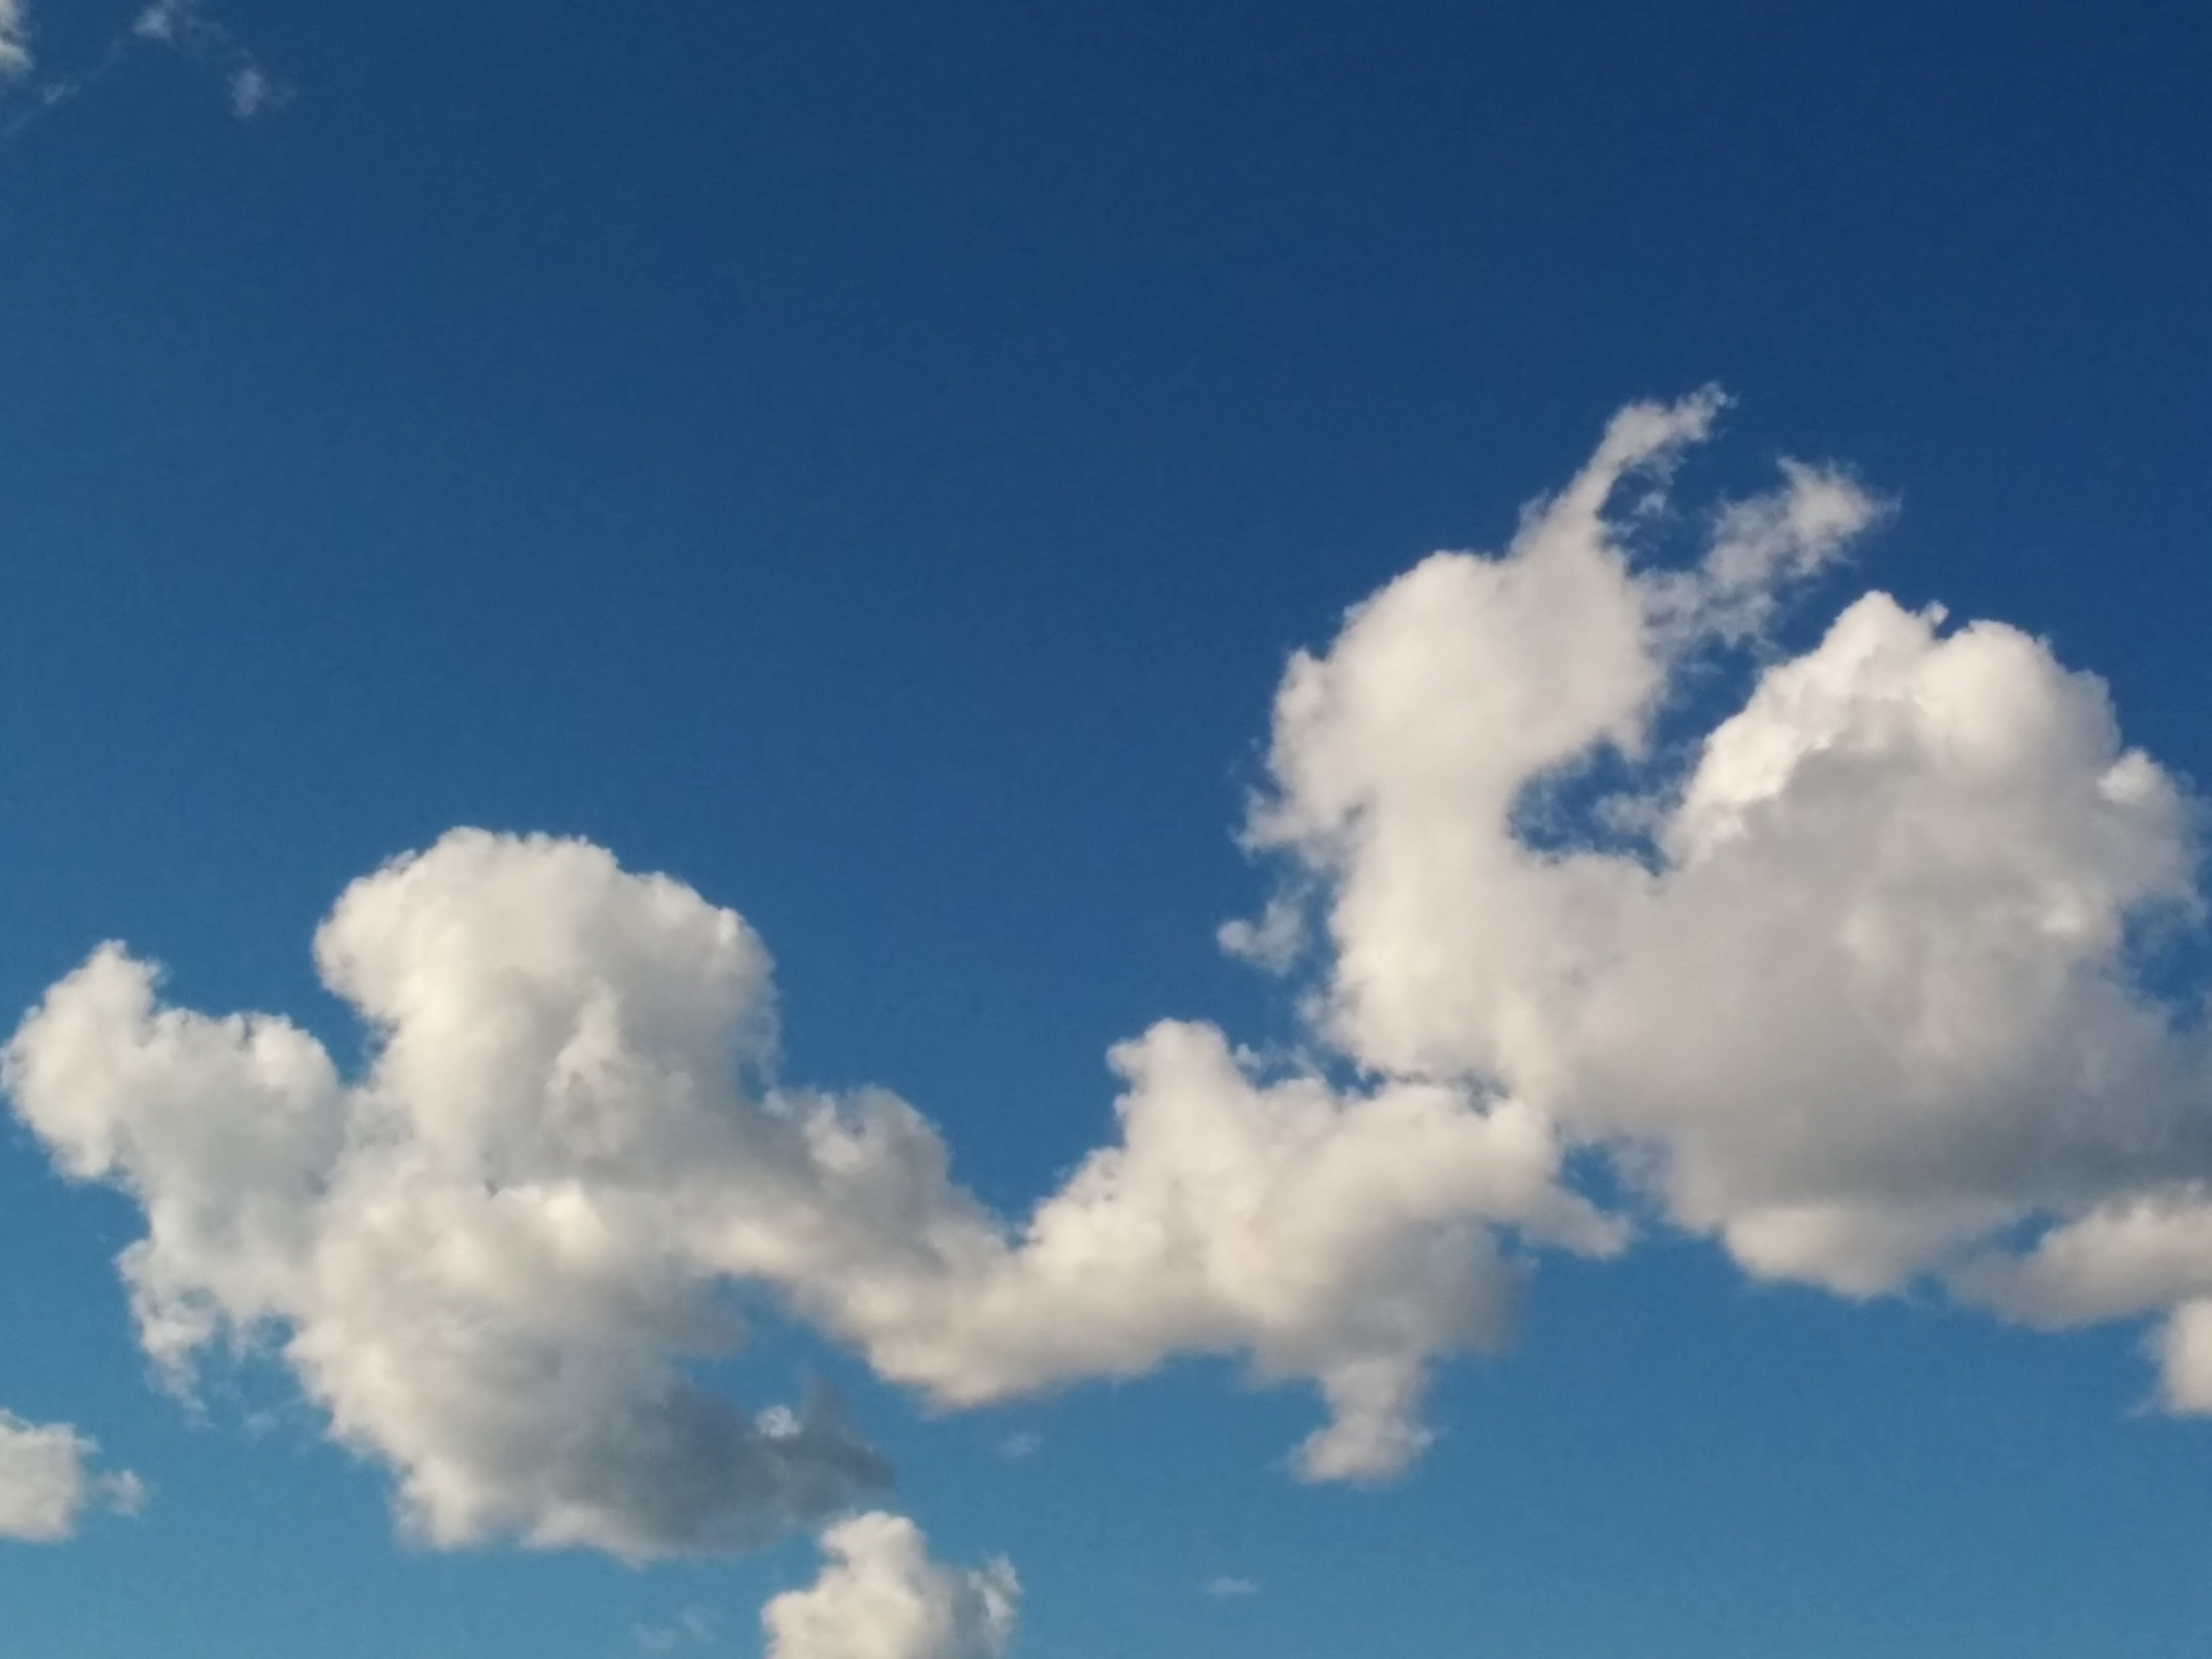
\includegraphics[width=0.9\textwidth,height=5cm]{gfx/images/stock-clouds}
	\caption[Results: Varying Scrambler Initialization for 1000 experiments]{Results: Varying Scrambler Initialization for 1000 experiments at MCS 0}
	\label{fig:vary_scrambler}
\end{figure}


%% -----------------------------------------------------------------------------

\section{Preceeding Data Variations}\label{sec:ex-destination}

Similarly to the scrambler initialization, the MAC header field preceeding the sender MAC address could also influence detection quality. This is due to the convolutional encoder as described in section \ref{sec:mac-and-phy}. The field before the sender MAC address in a data frame is the destination MAC address. In the following experiment, I measured to which extent the value of the destination address affects the accuracy of my detection technique.\\

Figure \ref{fig:vary_dest} shows the results in the same way as for the previous figures. Since the convolutional encoder uses a 7 bit state, only the last 7 bits of the destination MAC address matter. After these last 7 bits, the register is synchronized to the same state, regardless of the preceeding first 41 bits of the address. This makes up for a total of 128 different values that are evaluated with 1000 experiments each. As for the scrambler initialitation, the experiments are done at \gls{MCS} 0.

\begin{figure}[H]
	\centering
	% uncomment the following line to recompile the figure when it changes otherwise a cached version is used
	%\tikzset{external/remake next}
	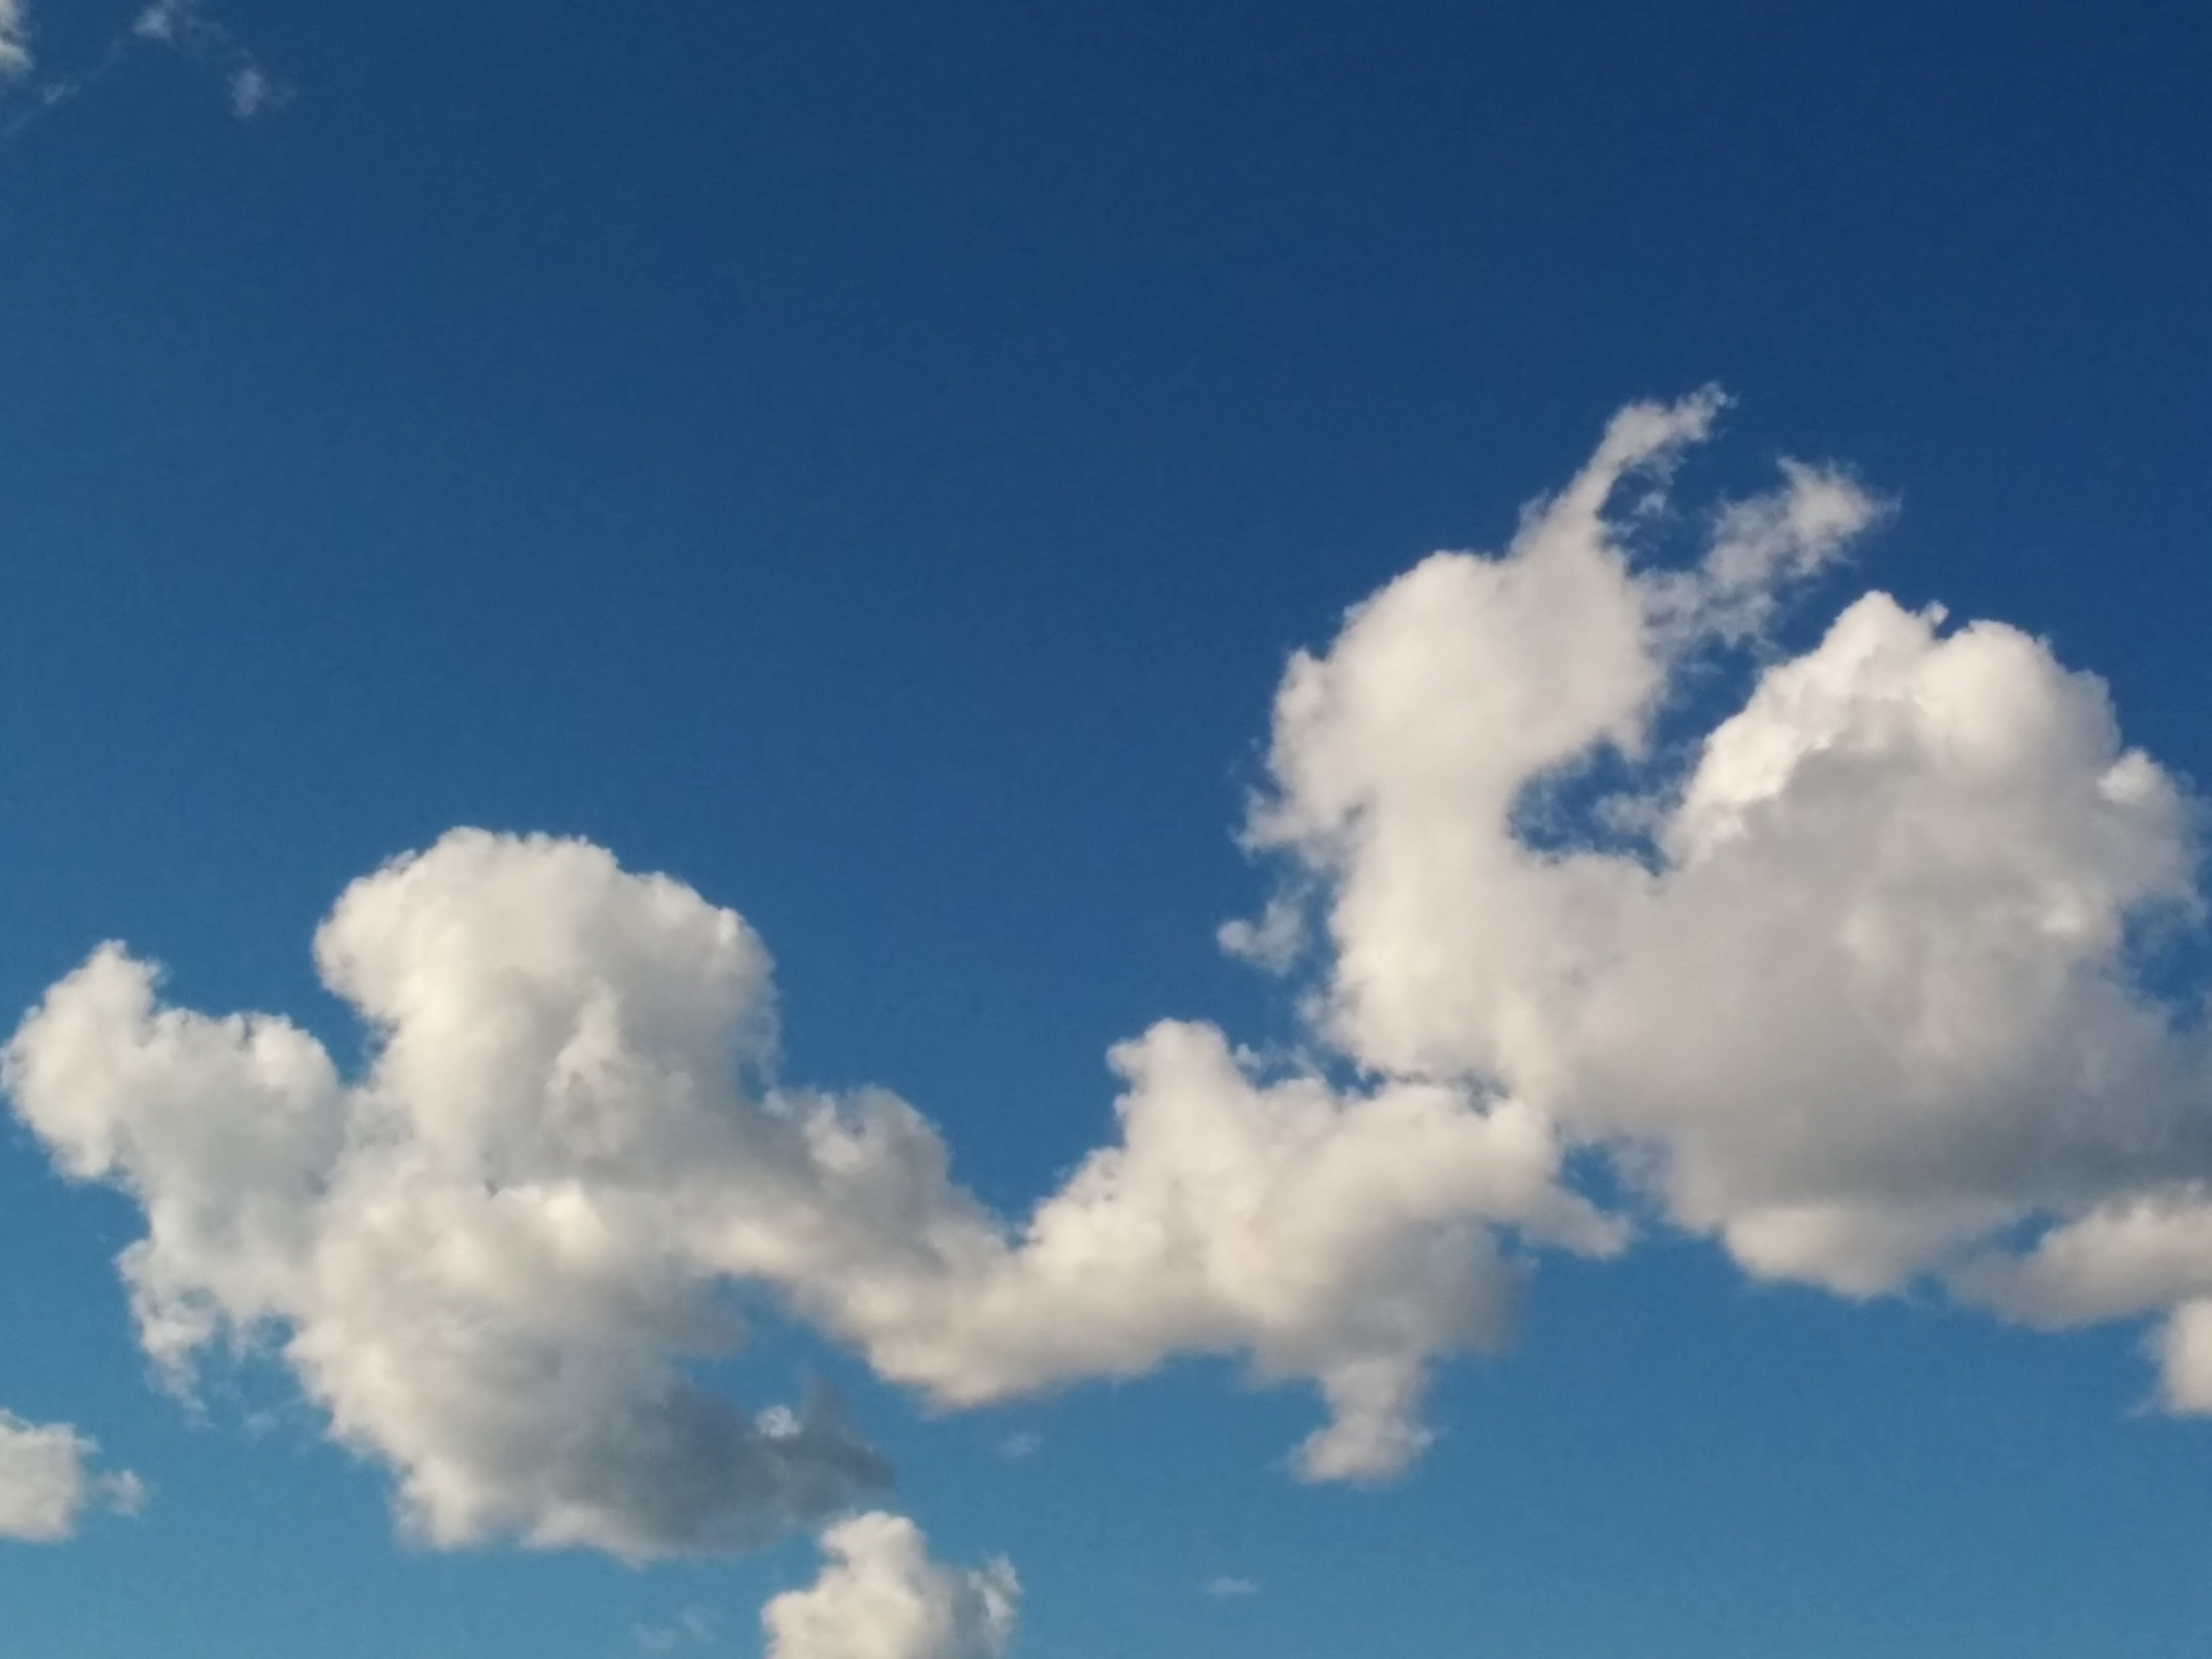
\includegraphics[width=0.9\textwidth,height=5cm]{gfx/images/stock-clouds}
	\caption[Results: Varying Destination MAC Address for 1000 experiments]{Results: Varying Destination MAC Address for 1000 experiments at MCS 0}
	\label{fig:vary_dest}
\end{figure}

It turns out that unlike the scrambler initialization, preceeding payload data does not really have a measurable effect. Detection quality is comparable regardless of the trailing bits of the MAC address. I discuss possible reasons for this in section \ref{sec:detection-quality}. An important implication of this result is that it is not necessary to check all 128 possible encoder states for every collision in real-time, which would be another linear scaling factor for the computational complexity of the algorithm.


%% -----------------------------------------------------------------------------

\section{Channel Models}

So far, all experiments were done in simulations with an ideal channel, meaning there were no path effects such as multi-path fading or attenuation. As this is not very realistic, I will evaluate performance under various channel models in this section.\\

Using Matlab, there are different models available that could be applied. On the one hand, the Communications System Toolbox comes with \texttt{stdchan}, which supports the \texttt{802.11g} and \texttt{802.11g} channel types. These are suited quite well for this scenario. The channel models requires some parameters, including the sampling frequency, doppler spread, and \gls{RMS} delay spread $ t_{RMS} $. The delay spread was varied from 100 ns to 500 ns in steps of 50 ns. The usage of the stdchan filter is illustrated by listing \ref{lst:stdchan}:

\begin{lstlisting}[captionpos=b,caption={Matlab stdchan Channel Model},label=lst:stdchan]
tmrs = ...;
fs = 20e6; % Hz Sampling Frequency
fd = 10; % Hz Doppler spread
chan = stdchan(1/fs, fd, '802.11g', trms);
rx = filter(chan, tx);
\end{lstlisting}

The results of this experiment are shown in figure \ref{fig:vary_trms}. For every trms value, 1000 experiments were conducted. The process was repeated for all eight \glspl{MCS}.

On the other hand, the WLAN Systems Toolbox comes with a number of specifically drafted IEEE 802.11 channel models. These are designed according to the IEEE 802.11 standard models described in the specification \cite{ieee2012}. There are 6 models (A to F), of which I used the following three:

\begin{itemize}
	\item \textit{Model B}: typical large open space and office environments, no line-of-sight, 100 ns RMS delay spread
	\item \textit{Model D}: large open space (indoor and outdoor), line-of-sight conditions, 140 ns RMS delay spread
	\item \textit{Model E}: typical large open space (indoor and outdoor), no line-of-sight, 250 ns RMS delay spread
\end{itemize}

I use the \texttt{wlanTGnChannel} class. Technically, this channel is designed to be used with IEEE 802.11 n high-troughput networks. However, the class supports configuration of MIMO streams. I set those to 1 antenna for transmission and reception, respectively. This should provide appropriate conditions for SISO 802.11 a/g networks.

The channel is used with Matlab code similar to listing \ref{lst:tgn}. As for the \texttt{stdchan} invocation, the sampling rate must be passed to the function. I use pathloss and shadowing for fading, and configure SISO.

\begin{lstlisting}[captionpos=b,caption={Matlab wlanTGnChannel Simulation},label=lst:tgn]
model = ...; % 'Model-B', 'Model-D', etc.
tgnchan = wlanTGnChannel( ...
        'SampleRate', 20e6, ... % Hz
        'LargeScaleFadingEffect', 'Pathloss and shadowing', ...
        'NumTransmitAntennas', 1, 'NumReceiveAntennas', 1, ... % SISO
        'DelayProfile', model);
rx = tgnchan(tx);
\end{lstlisting}

The results of the experiments are shown in figure \ref{fig:vary_tgn}. For each of the three channel models, 1000 experiments were conducted at each \gls{MCS}.

\begin{figure}[p]
	\centering
	\setlength\figureheight{3cm}
	\setlength\figurewidth{0.40\textwidth}
	\begin{tabular}{cc}
		% uncomment the following line to recompile the figure when it changes otherwise a cached version is used
		%\tikzset{external/remake next}
		\subfloat[MCS 0]{% This file was created by matlab2tikz.
%
%The latest updates can be retrieved from
%  http://www.mathworks.com/matlabcentral/fileexchange/22022-matlab2tikz-matlab2tikz
%where you can also make suggestions and rate matlab2tikz.
%
\definecolor{mycolor1}{rgb}{0.24220,0.15040,0.66030}%
\definecolor{mycolor2}{rgb}{0.09640,0.75000,0.71204}%
\definecolor{mycolor3}{rgb}{0.97690,0.98390,0.08050}%
%
\begin{tikzpicture}[%
font=\footnotesize
]

\begin{axis}[%
width=0.951\figurewidth,
height=\figureheight,
at={(0\figurewidth,0\figureheight)},
scale only axis,
bar width=0,
xmin=5e-08,
xmax=5.5e-07,
xlabel style={font=\color{white!15!black}},
xlabel={$\text{802.11g stdchan: t}_\text{R}\text{MS in seconds}$},
ymin=0,
ymax=10,
ylabel style={font=\color{white!15!black}},
ylabel={\# experiments},
axis background/.style={fill=white},
title style={font=\bfseries},
title={MCS 0},
legend style={legend cell align=left, align=left, draw=white!15!black},
clip mode=individual,transpose legend,legend columns=2,legend style={at={(0,1)},anchor=north west,draw=black,fill=white,legend cell align=left}
]
\addplot[ybar stacked, fill=mycolor1, draw=black, area legend] table[row sep=crcr] {%
1e-07	0\\
1.5e-07	0\\
2e-07	0\\
2.5e-07	0\\
3e-07	0\\
3.5e-07	0\\
4e-07	0\\
4.5e-07	0\\
5e-07	0\\
};
\addplot[forget plot, color=white!15!black] table[row sep=crcr] {%
5e-08	0\\
5.5e-07	0\\
};
\addlegendentry{0 correct}

\addplot[ybar stacked, fill=mycolor2, draw=black, area legend] table[row sep=crcr] {%
1e-07	5\\
1.5e-07	3\\
2e-07	8\\
2.5e-07	4\\
3e-07	6\\
3.5e-07	7\\
4e-07	8\\
4.5e-07	7\\
5e-07	7\\
};
\addplot[forget plot, color=white!15!black] table[row sep=crcr] {%
5e-08	0\\
5.5e-07	0\\
};
\addlegendentry{1 correct}

\addplot[ybar stacked, fill=mycolor3, draw=black, area legend] table[row sep=crcr] {%
1e-07	5\\
1.5e-07	7\\
2e-07	2\\
2.5e-07	6\\
3e-07	4\\
3.5e-07	3\\
4e-07	2\\
4.5e-07	3\\
5e-07	3\\
};
\addplot[forget plot, color=white!15!black] table[row sep=crcr]  &
		\subfloat[MCS 1]{% This file was created by matlab2tikz.
%
%The latest updates can be retrieved from
%  http://www.mathworks.com/matlabcentral/fileexchange/22022-matlab2tikz-matlab2tikz
%where you can also make suggestions and rate matlab2tikz.
%
\definecolor{mycolor1}{rgb}{0.24220,0.15040,0.66030}%
\definecolor{mycolor2}{rgb}{0.09640,0.75000,0.71204}%
\definecolor{mycolor3}{rgb}{0.97690,0.98390,0.08050}%
%
\begin{tikzpicture}[%
font=\footnotesize
]

\begin{axis}[%
width=0.951\figurewidth,
height=\figureheight,
at={(0\figurewidth,0\figureheight)},
scale only axis,
bar width=0,
xmin=5e-08,
xmax=5.5e-07,
xlabel style={font=\color{white!15!black}},
xlabel={$\text{802.11g stdchan: t}_\text{R}\text{MS in seconds}$},
ymin=0,
ymax=10,
ylabel style={font=\color{white!15!black}},
ylabel={\# experiments},
axis background/.style={fill=white},
title style={font=\bfseries},
title={MCS 1},
legend style={legend cell align=left, align=left, draw=white!15!black},
clip mode=individual,transpose legend,legend columns=2,legend style={at={(0,1)},anchor=north west,draw=black,fill=white,legend cell align=left}
]
\addplot[ybar stacked, fill=mycolor1, draw=black, area legend] table[row sep=crcr] {%
1e-07	0\\
1.5e-07	0\\
2e-07	0\\
2.5e-07	1\\
3e-07	4\\
3.5e-07	2\\
4e-07	6\\
4.5e-07	5\\
5e-07	4\\
};
\addplot[forget plot, color=white!15!black] table[row sep=crcr] {%
5e-08	0\\
5.5e-07	0\\
};
\addlegendentry{0 correct}

\addplot[ybar stacked, fill=mycolor2, draw=black, area legend] table[row sep=crcr] {%
1e-07	6\\
1.5e-07	6\\
2e-07	10\\
2.5e-07	7\\
3e-07	5\\
3.5e-07	7\\
4e-07	3\\
4.5e-07	5\\
5e-07	5\\
};
\addplot[forget plot, color=white!15!black] table[row sep=crcr] {%
5e-08	0\\
5.5e-07	0\\
};
\addlegendentry{1 correct}

\addplot[ybar stacked, fill=mycolor3, draw=black, area legend] table[row sep=crcr] {%
1e-07	4\\
1.5e-07	4\\
2e-07	0\\
2.5e-07	2\\
3e-07	1\\
3.5e-07	1\\
4e-07	1\\
4.5e-07	0\\
5e-07	1\\
};
\addplot[forget plot, color=white!15!black] table[row sep=crcr]  \\
		\subfloat[MCS 2]{% This file was created by matlab2tikz.
%
%The latest updates can be retrieved from
%  http://www.mathworks.com/matlabcentral/fileexchange/22022-matlab2tikz-matlab2tikz
%where you can also make suggestions and rate matlab2tikz.
%
\definecolor{mycolor1}{rgb}{0.24220,0.15040,0.66030}%
\definecolor{mycolor2}{rgb}{0.09640,0.75000,0.71204}%
\definecolor{mycolor3}{rgb}{0.97690,0.98390,0.08050}%
%
\begin{tikzpicture}[%
font=\footnotesize
]

\begin{axis}[%
width=0.951\figurewidth,
height=\figureheight,
at={(0\figurewidth,0\figureheight)},
scale only axis,
bar width=0,
xmin=5e-08,
xmax=5.5e-07,
xlabel style={font=\color{white!15!black}},
xlabel={$\text{802.11g stdchan: t}_\text{R}\text{MS in seconds}$},
ymin=0,
ymax=10,
ylabel style={font=\color{white!15!black}},
ylabel={\# experiments},
axis background/.style={fill=white},
title style={font=\bfseries},
title={MCS 2},
legend style={legend cell align=left, align=left, draw=white!15!black},
clip mode=individual,transpose legend,legend columns=2,legend style={at={(0,1)},anchor=north west,draw=black,fill=white,legend cell align=left}
]
\addplot[ybar stacked, fill=mycolor1, draw=black, area legend] table[row sep=crcr] {%
1e-07	0\\
1.5e-07	0\\
2e-07	0\\
2.5e-07	0\\
3e-07	1\\
3.5e-07	4\\
4e-07	1\\
4.5e-07	3\\
5e-07	3\\
};
\addplot[forget plot, color=white!15!black] table[row sep=crcr] {%
5e-08	0\\
5.5e-07	0\\
};
\addlegendentry{0 correct}

\addplot[ybar stacked, fill=mycolor2, draw=black, area legend] table[row sep=crcr] {%
1e-07	7\\
1.5e-07	7\\
2e-07	9\\
2.5e-07	9\\
3e-07	7\\
3.5e-07	5\\
4e-07	7\\
4.5e-07	6\\
5e-07	7\\
};
\addplot[forget plot, color=white!15!black] table[row sep=crcr] {%
5e-08	0\\
5.5e-07	0\\
};
\addlegendentry{1 correct}

\addplot[ybar stacked, fill=mycolor3, draw=black, area legend] table[row sep=crcr] {%
1e-07	3\\
1.5e-07	3\\
2e-07	1\\
2.5e-07	1\\
3e-07	2\\
3.5e-07	1\\
4e-07	2\\
4.5e-07	1\\
5e-07	0\\
};
\addplot[forget plot, color=white!15!black] table[row sep=crcr]  &
		\subfloat[MCS 3]{% This file was created by matlab2tikz.
%
%The latest updates can be retrieved from
%  http://www.mathworks.com/matlabcentral/fileexchange/22022-matlab2tikz-matlab2tikz
%where you can also make suggestions and rate matlab2tikz.
%
\definecolor{mycolor1}{rgb}{0.24220,0.15040,0.66030}%
\definecolor{mycolor2}{rgb}{0.09640,0.75000,0.71204}%
\definecolor{mycolor3}{rgb}{0.97690,0.98390,0.08050}%
%
\begin{tikzpicture}[%
font=\footnotesize
]

\begin{axis}[%
width=0.951\figurewidth,
height=\figureheight,
at={(0\figurewidth,0\figureheight)},
scale only axis,
bar width=0,
xmin=5e-08,
xmax=5.5e-07,
xlabel style={font=\color{white!15!black}},
xlabel={$\text{802.11g stdchan: t}_\text{R}\text{MS in seconds}$},
ymin=0,
ymax=10,
ylabel style={font=\color{white!15!black}},
ylabel={\# experiments},
axis background/.style={fill=white},
title style={font=\bfseries},
title={MCS 3},
legend style={legend cell align=left, align=left, draw=white!15!black},
clip mode=individual,transpose legend,legend columns=2,legend style={at={(0,1)},anchor=north west,draw=black,fill=white,legend cell align=left}
]
\addplot[ybar stacked, fill=mycolor1, draw=black, area legend] table[row sep=crcr] {%
1e-07	1\\
1.5e-07	6\\
2e-07	2\\
2.5e-07	4\\
3e-07	4\\
3.5e-07	6\\
4e-07	6\\
4.5e-07	6\\
5e-07	6\\
};
\addplot[forget plot, color=white!15!black] table[row sep=crcr] {%
5e-08	0\\
5.5e-07	0\\
};
\addlegendentry{0 correct}

\addplot[ybar stacked, fill=mycolor2, draw=black, area legend] table[row sep=crcr] {%
1e-07	7\\
1.5e-07	2\\
2e-07	6\\
2.5e-07	6\\
3e-07	6\\
3.5e-07	4\\
4e-07	4\\
4.5e-07	4\\
5e-07	4\\
};
\addplot[forget plot, color=white!15!black] table[row sep=crcr] {%
5e-08	0\\
5.5e-07	0\\
};
\addlegendentry{1 correct}

\addplot[ybar stacked, fill=mycolor3, draw=black, area legend] table[row sep=crcr] {%
1e-07	2\\
1.5e-07	2\\
2e-07	2\\
2.5e-07	0\\
3e-07	0\\
3.5e-07	0\\
4e-07	0\\
4.5e-07	0\\
5e-07	0\\
};
\addplot[forget plot, color=white!15!black] table[row sep=crcr]  \\
		\subfloat[MCS 4]{% This file was created by matlab2tikz.
%
%The latest updates can be retrieved from
%  http://www.mathworks.com/matlabcentral/fileexchange/22022-matlab2tikz-matlab2tikz
%where you can also make suggestions and rate matlab2tikz.
%
\definecolor{mycolor1}{rgb}{0.24220,0.15040,0.66030}%
\definecolor{mycolor2}{rgb}{0.09640,0.75000,0.71204}%
\definecolor{mycolor3}{rgb}{0.97690,0.98390,0.08050}%
%
\begin{tikzpicture}[%
font=\footnotesize
]

\begin{axis}[%
width=0.951\figurewidth,
height=\figureheight,
at={(0\figurewidth,0\figureheight)},
scale only axis,
bar width=0,
xmin=5e-08,
xmax=5.5e-07,
xlabel style={font=\color{white!15!black}},
xlabel={$\text{802.11g stdchan: t}_\text{R}\text{MS in seconds}$},
ymin=0,
ymax=10,
ylabel style={font=\color{white!15!black}},
ylabel={\# experiments},
axis background/.style={fill=white},
title style={font=\bfseries},
title={MCS 4},
legend style={legend cell align=left, align=left, draw=white!15!black},
clip mode=individual,transpose legend,legend columns=2,legend style={at={(0,1)},anchor=north west,draw=black,fill=white,legend cell align=left}
]
\addplot[ybar stacked, fill=mycolor1, draw=black, area legend] table[row sep=crcr] {%
1e-07	4\\
1.5e-07	6\\
2e-07	4\\
2.5e-07	4\\
3e-07	7\\
3.5e-07	7\\
4e-07	7\\
4.5e-07	7\\
5e-07	8\\
};
\addplot[forget plot, color=white!15!black] table[row sep=crcr] {%
5e-08	0\\
5.5e-07	0\\
};
\addlegendentry{0 correct}

\addplot[ybar stacked, fill=mycolor2, draw=black, area legend] table[row sep=crcr] {%
1e-07	4\\
1.5e-07	4\\
2e-07	6\\
2.5e-07	5\\
3e-07	3\\
3.5e-07	2\\
4e-07	3\\
4.5e-07	3\\
5e-07	2\\
};
\addplot[forget plot, color=white!15!black] table[row sep=crcr] {%
5e-08	0\\
5.5e-07	0\\
};
\addlegendentry{1 correct}

\addplot[ybar stacked, fill=mycolor3, draw=black, area legend] table[row sep=crcr] {%
1e-07	2\\
1.5e-07	0\\
2e-07	0\\
2.5e-07	1\\
3e-07	0\\
3.5e-07	1\\
4e-07	0\\
4.5e-07	0\\
5e-07	0\\
};
\addplot[forget plot, color=white!15!black] table[row sep=crcr]  &
		\subfloat[MCS 5]{% This file was created by matlab2tikz.
%
%The latest updates can be retrieved from
%  http://www.mathworks.com/matlabcentral/fileexchange/22022-matlab2tikz-matlab2tikz
%where you can also make suggestions and rate matlab2tikz.
%
\definecolor{mycolor1}{rgb}{0.24220,0.15040,0.66030}%
\definecolor{mycolor2}{rgb}{0.09640,0.75000,0.71204}%
\definecolor{mycolor3}{rgb}{0.97690,0.98390,0.08050}%
%
\begin{tikzpicture}[%
font=\footnotesize
]

\begin{axis}[%
width=0.951\figurewidth,
height=\figureheight,
at={(0\figurewidth,0\figureheight)},
scale only axis,
bar width=0,
xmin=5e-08,
xmax=5.5e-07,
xlabel style={font=\color{white!15!black}},
xlabel={$\text{802.11g stdchan: t}_\text{R}\text{MS in seconds}$},
ymin=0,
ymax=10,
ylabel style={font=\color{white!15!black}},
ylabel={\# experiments},
axis background/.style={fill=white},
title style={font=\bfseries},
title={MCS 5},
legend style={legend cell align=left, align=left, draw=white!15!black},
clip mode=individual,transpose legend,legend columns=2,legend style={at={(0,1)},anchor=north west,draw=black,fill=white,legend cell align=left}
]
\addplot[ybar stacked, fill=mycolor1, draw=black, area legend] table[row sep=crcr] {%
1e-07	0\\
1.5e-07	4\\
2e-07	3\\
2.5e-07	3\\
3e-07	4\\
3.5e-07	9\\
4e-07	4\\
4.5e-07	7\\
5e-07	8\\
};
\addplot[forget plot, color=white!15!black] table[row sep=crcr] {%
5e-08	0\\
5.5e-07	0\\
};
\addlegendentry{0 correct}

\addplot[ybar stacked, fill=mycolor2, draw=black, area legend] table[row sep=crcr] {%
1e-07	8\\
1.5e-07	6\\
2e-07	5\\
2.5e-07	6\\
3e-07	5\\
3.5e-07	1\\
4e-07	6\\
4.5e-07	3\\
5e-07	2\\
};
\addplot[forget plot, color=white!15!black] table[row sep=crcr] {%
5e-08	0\\
5.5e-07	0\\
};
\addlegendentry{1 correct}

\addplot[ybar stacked, fill=mycolor3, draw=black, area legend] table[row sep=crcr] {%
1e-07	2\\
1.5e-07	0\\
2e-07	2\\
2.5e-07	1\\
3e-07	1\\
3.5e-07	0\\
4e-07	0\\
4.5e-07	0\\
5e-07	0\\
};
\addplot[forget plot, color=white!15!black] table[row sep=crcr]  \\
		\subfloat[MCS 6]{% This file was created by matlab2tikz.
%
%The latest updates can be retrieved from
%  http://www.mathworks.com/matlabcentral/fileexchange/22022-matlab2tikz-matlab2tikz
%where you can also make suggestions and rate matlab2tikz.
%
\definecolor{mycolor1}{rgb}{0.24220,0.15040,0.66030}%
\definecolor{mycolor2}{rgb}{0.09640,0.75000,0.71204}%
\definecolor{mycolor3}{rgb}{0.97690,0.98390,0.08050}%
%
\begin{tikzpicture}[%
font=\footnotesize
]

\begin{axis}[%
width=0.951\figurewidth,
height=\figureheight,
at={(0\figurewidth,0\figureheight)},
scale only axis,
bar width=0,
xmin=5e-08,
xmax=5.5e-07,
xlabel style={font=\color{white!15!black}},
xlabel={$\text{802.11g stdchan: t}_\text{R}\text{MS in seconds}$},
ymin=0,
ymax=10,
ylabel style={font=\color{white!15!black}},
ylabel={\# experiments},
axis background/.style={fill=white},
title style={font=\bfseries},
title={MCS 6},
legend style={legend cell align=left, align=left, draw=white!15!black},
clip mode=individual,transpose legend,legend columns=2,legend style={at={(0,1)},anchor=north west,draw=black,fill=white,legend cell align=left}
]
\addplot[ybar stacked, fill=mycolor1, draw=black, area legend] table[row sep=crcr] {%
1e-07	5\\
1.5e-07	8\\
2e-07	6\\
2.5e-07	8\\
3e-07	7\\
3.5e-07	7\\
4e-07	8\\
4.5e-07	8\\
5e-07	6\\
};
\addplot[forget plot, color=white!15!black] table[row sep=crcr] {%
5e-08	0\\
5.5e-07	0\\
};
\addlegendentry{0 correct}

\addplot[ybar stacked, fill=mycolor2, draw=black, area legend] table[row sep=crcr] {%
1e-07	4\\
1.5e-07	2\\
2e-07	4\\
2.5e-07	2\\
3e-07	3\\
3.5e-07	3\\
4e-07	2\\
4.5e-07	2\\
5e-07	4\\
};
\addplot[forget plot, color=white!15!black] table[row sep=crcr] {%
5e-08	0\\
5.5e-07	0\\
};
\addlegendentry{1 correct}

\addplot[ybar stacked, fill=mycolor3, draw=black, area legend] table[row sep=crcr] {%
1e-07	1\\
1.5e-07	0\\
2e-07	0\\
2.5e-07	0\\
3e-07	0\\
3.5e-07	0\\
4e-07	0\\
4.5e-07	0\\
5e-07	0\\
};
\addplot[forget plot, color=white!15!black] table[row sep=crcr]  &
		\subfloat[MCS 7]{% This file was created by matlab2tikz.
%
%The latest updates can be retrieved from
%  http://www.mathworks.com/matlabcentral/fileexchange/22022-matlab2tikz-matlab2tikz
%where you can also make suggestions and rate matlab2tikz.
%
\definecolor{mycolor1}{rgb}{0.24220,0.15040,0.66030}%
\definecolor{mycolor2}{rgb}{0.09640,0.75000,0.71204}%
\definecolor{mycolor3}{rgb}{0.97690,0.98390,0.08050}%
%
\begin{tikzpicture}[%
font=\footnotesize
]

\begin{axis}[%
width=0.951\figurewidth,
height=\figureheight,
at={(0\figurewidth,0\figureheight)},
scale only axis,
bar width=0,
xmin=5e-08,
xmax=5.5e-07,
xlabel style={font=\color{white!15!black}},
xlabel={$\text{802.11g stdchan: t}_\text{R}\text{MS in seconds}$},
ymin=0,
ymax=10,
ylabel style={font=\color{white!15!black}},
ylabel={\# experiments},
axis background/.style={fill=white},
title style={font=\bfseries},
title={MCS 7},
legend style={legend cell align=left, align=left, draw=white!15!black},
clip mode=individual,transpose legend,legend columns=2,legend style={at={(0,1)},anchor=north west,draw=black,fill=white,legend cell align=left}
]
\addplot[ybar stacked, fill=mycolor1, draw=black, area legend] table[row sep=crcr] {%
1e-07	8\\
1.5e-07	7\\
2e-07	7\\
2.5e-07	8\\
3e-07	9\\
3.5e-07	10\\
4e-07	10\\
4.5e-07	8\\
5e-07	10\\
};
\addplot[forget plot, color=white!15!black] table[row sep=crcr] {%
5e-08	0\\
5.5e-07	0\\
};
\addlegendentry{0 correct}

\addplot[ybar stacked, fill=mycolor2, draw=black, area legend] table[row sep=crcr] {%
1e-07	2\\
1.5e-07	3\\
2e-07	3\\
2.5e-07	2\\
3e-07	1\\
3.5e-07	0\\
4e-07	0\\
4.5e-07	2\\
5e-07	0\\
};
\addplot[forget plot, color=white!15!black] table[row sep=crcr] {%
5e-08	0\\
5.5e-07	0\\
};
\addlegendentry{1 correct}

\addplot[ybar stacked, fill=mycolor3, draw=black, area legend] table[row sep=crcr] {%
1e-07	0\\
1.5e-07	0\\
2e-07	0\\
2.5e-07	0\\
3e-07	0\\
3.5e-07	0\\
4e-07	0\\
4.5e-07	0\\
5e-07	0\\
};
\addplot[forget plot, color=white!15!black] table[row sep=crcr]  \\
	\end{tabular}
	\caption{Results: Varying $t_{RMS}$ in a Standard Channel for 1000 Experiments}
	\label{fig:vary_trms}
\end{figure}

\begin{figure}[p]
	\centering
	\setlength\figureheight{3cm}
	\setlength\figurewidth{0.40\textwidth}
	\begin{tabular}{cc}
		% uncomment the following line to recompile the figure when it changes otherwise a cached version is used
		%\tikzset{external/remake next}
		\subfloat[MCS 0]{% This file was created by matlab2tikz.
%
%The latest updates can be retrieved from
%  http://www.mathworks.com/matlabcentral/fileexchange/22022-matlab2tikz-matlab2tikz
%where you can also make suggestions and rate matlab2tikz.
%
\definecolor{mycolor1}{rgb}{0.24220,0.15040,0.66030}%
\definecolor{mycolor2}{rgb}{0.09640,0.75000,0.71204}%
\definecolor{mycolor3}{rgb}{0.97690,0.98390,0.08050}%
%
\begin{tikzpicture}[%
font=\footnotesize
]

\begin{axis}[%
width=0.951\figurewidth,
height=\figureheight,
at={(0\figurewidth,0\figureheight)},
scale only axis,
bar width=0.8,
xmin=0.5,
xmax=3.5,
xtick={1,2,3},
xticklabels={{Model-B},{Model-D},{Model-E}},
xlabel style={font=\color{white!15!black}},
xlabel={AGWN SNR},
ymin=0,
ymax=100,
ylabel style={font=\color{white!15!black}},
ylabel={\# experiments},
axis background/.style={fill=white},
title style={font=\bfseries},
title={MCS 0},
legend style={legend cell align=left, align=left, draw=white!15!black},
clip mode=individual,transpose legend,legend columns=2,legend style={at={(0,1)},anchor=north west,draw=black,fill=white,legend cell align=left}
]
\addplot[ybar stacked, fill=mycolor1, draw=black, area legend] table[row sep=crcr] {%
1	0\\
2	0\\
3	0\\
};
\addplot[forget plot, color=white!15!black] table[row sep=crcr] {%
0.5	0\\
3.5	0\\
};
\addlegendentry{0 correct}

\addplot[ybar stacked, fill=mycolor2, draw=black, area legend] table[row sep=crcr] {%
1	0\\
2	0\\
3	1\\
};
\addplot[forget plot, color=white!15!black] table[row sep=crcr] {%
0.5	0\\
3.5	0\\
};
\addlegendentry{1 correct}

\addplot[ybar stacked, fill=mycolor3, draw=black, area legend] table[row sep=crcr] {%
1	100\\
2	100\\
3	99\\
};
\addplot[forget plot, color=white!15!black] table[row sep=crcr]  &
		\subfloat[MCS 1]{% This file was created by matlab2tikz.
%
%The latest updates can be retrieved from
%  http://www.mathworks.com/matlabcentral/fileexchange/22022-matlab2tikz-matlab2tikz
%where you can also make suggestions and rate matlab2tikz.
%
\definecolor{mycolor1}{rgb}{0.24220,0.15040,0.66030}%
\definecolor{mycolor2}{rgb}{0.09640,0.75000,0.71204}%
\definecolor{mycolor3}{rgb}{0.97690,0.98390,0.08050}%
%
\begin{tikzpicture}[%
font=\footnotesize
]

\begin{axis}[%
width=0.951\figurewidth,
height=\figureheight,
at={(0\figurewidth,0\figureheight)},
scale only axis,
bar width=0.8,
xmin=0.5,
xmax=3.5,
xtick={1,2,3},
xticklabels={{Model-B},{Model-D},{Model-E}},
xlabel style={font=\color{white!15!black}},
xlabel={AGWN SNR},
ymin=0,
ymax=100,
ylabel style={font=\color{white!15!black}},
ylabel={\# experiments},
axis background/.style={fill=white},
title style={font=\bfseries},
title={MCS 1},
legend style={legend cell align=left, align=left, draw=white!15!black},
clip mode=individual,transpose legend,legend columns=2,legend style={at={(0,1)},anchor=north west,draw=black,fill=white,legend cell align=left}
]
\addplot[ybar stacked, fill=mycolor1, draw=black, area legend] table[row sep=crcr] {%
1	5\\
2	7\\
3	13\\
};
\addplot[forget plot, color=white!15!black] table[row sep=crcr] {%
0.5	0\\
3.5	0\\
};
\addlegendentry{0 correct}

\addplot[ybar stacked, fill=mycolor2, draw=black, area legend] table[row sep=crcr] {%
1	1\\
2	2\\
3	3\\
};
\addplot[forget plot, color=white!15!black] table[row sep=crcr] {%
0.5	0\\
3.5	0\\
};
\addlegendentry{1 correct}

\addplot[ybar stacked, fill=mycolor3, draw=black, area legend] table[row sep=crcr] {%
1	94\\
2	91\\
3	84\\
};
\addplot[forget plot, color=white!15!black] table[row sep=crcr]  \\
		\subfloat[MCS 2]{% This file was created by matlab2tikz.
%
%The latest updates can be retrieved from
%  http://www.mathworks.com/matlabcentral/fileexchange/22022-matlab2tikz-matlab2tikz
%where you can also make suggestions and rate matlab2tikz.
%
\definecolor{mycolor1}{rgb}{0.24220,0.15040,0.66030}%
\definecolor{mycolor2}{rgb}{0.09640,0.75000,0.71204}%
\definecolor{mycolor3}{rgb}{0.97690,0.98390,0.08050}%
%
\begin{tikzpicture}[%
font=\footnotesize
]

\begin{axis}[%
width=0.951\figurewidth,
height=\figureheight,
at={(0\figurewidth,0\figureheight)},
scale only axis,
bar width=0.8,
xmin=0.5,
xmax=3.5,
xtick={1,2,3},
xticklabels={{Model-B},{Model-D},{Model-E}},
xlabel style={font=\color{white!15!black}},
xlabel={AGWN SNR},
ymin=0,
ymax=100,
ylabel style={font=\color{white!15!black}},
ylabel={\# experiments},
axis background/.style={fill=white},
title style={font=\bfseries},
title={MCS 2},
legend style={legend cell align=left, align=left, draw=white!15!black},
clip mode=individual,transpose legend,legend columns=2,legend style={at={(0,1)},anchor=north west,draw=black,fill=white,legend cell align=left}
]
\addplot[ybar stacked, fill=mycolor1, draw=black, area legend] table[row sep=crcr] {%
1	0\\
2	3\\
3	3\\
};
\addplot[forget plot, color=white!15!black] table[row sep=crcr] {%
0.5	0\\
3.5	0\\
};
\addlegendentry{0 correct}

\addplot[ybar stacked, fill=mycolor2, draw=black, area legend] table[row sep=crcr] {%
1	1\\
2	5\\
3	9\\
};
\addplot[forget plot, color=white!15!black] table[row sep=crcr] {%
0.5	0\\
3.5	0\\
};
\addlegendentry{1 correct}

\addplot[ybar stacked, fill=mycolor3, draw=black, area legend] table[row sep=crcr] {%
1	99\\
2	92\\
3	88\\
};
\addplot[forget plot, color=white!15!black] table[row sep=crcr]  &
		\subfloat[MCS 3]{% This file was created by matlab2tikz.
%
%The latest updates can be retrieved from
%  http://www.mathworks.com/matlabcentral/fileexchange/22022-matlab2tikz-matlab2tikz
%where you can also make suggestions and rate matlab2tikz.
%
\definecolor{mycolor1}{rgb}{0.24220,0.15040,0.66030}%
\definecolor{mycolor2}{rgb}{0.09640,0.75000,0.71204}%
\definecolor{mycolor3}{rgb}{0.97690,0.98390,0.08050}%
%
\begin{tikzpicture}[%
font=\footnotesize
]

\begin{axis}[%
width=0.951\figurewidth,
height=\figureheight,
at={(0\figurewidth,0\figureheight)},
scale only axis,
bar width=0.8,
xmin=0.5,
xmax=3.5,
xtick={1,2,3},
xticklabels={{Model-B},{Model-D},{Model-E}},
xlabel style={font=\color{white!15!black}},
xlabel={AGWN SNR},
ymin=0,
ymax=100,
ylabel style={font=\color{white!15!black}},
ylabel={\# experiments},
axis background/.style={fill=white},
title style={font=\bfseries},
title={MCS 3},
legend style={legend cell align=left, align=left, draw=white!15!black},
clip mode=individual,transpose legend,legend columns=2,legend style={at={(0,1)},anchor=north west,draw=black,fill=white,legend cell align=left}
]
\addplot[ybar stacked, fill=mycolor1, draw=black, area legend] table[row sep=crcr] {%
1	18\\
2	30\\
3	38\\
};
\addplot[forget plot, color=white!15!black] table[row sep=crcr] {%
0.5	0\\
3.5	0\\
};
\addlegendentry{0 correct}

\addplot[ybar stacked, fill=mycolor2, draw=black, area legend] table[row sep=crcr] {%
1	11\\
2	10\\
3	15\\
};
\addplot[forget plot, color=white!15!black] table[row sep=crcr] {%
0.5	0\\
3.5	0\\
};
\addlegendentry{1 correct}

\addplot[ybar stacked, fill=mycolor3, draw=black, area legend] table[row sep=crcr] {%
1	71\\
2	60\\
3	47\\
};
\addplot[forget plot, color=white!15!black] table[row sep=crcr]  \\
		\subfloat[MCS 4]{% This file was created by matlab2tikz.
%
%The latest updates can be retrieved from
%  http://www.mathworks.com/matlabcentral/fileexchange/22022-matlab2tikz-matlab2tikz
%where you can also make suggestions and rate matlab2tikz.
%
\definecolor{mycolor1}{rgb}{0.24220,0.15040,0.66030}%
\definecolor{mycolor2}{rgb}{0.09640,0.75000,0.71204}%
\definecolor{mycolor3}{rgb}{0.97690,0.98390,0.08050}%
%
\begin{tikzpicture}[%
font=\footnotesize
]

\begin{axis}[%
width=0.951\figurewidth,
height=\figureheight,
at={(0\figurewidth,0\figureheight)},
scale only axis,
bar width=0.8,
xmin=0.5,
xmax=3.5,
xtick={1,2,3},
xticklabels={{Model-B},{Model-D},{Model-E}},
xlabel style={font=\color{white!15!black}},
xlabel={AGWN SNR},
ymin=0,
ymax=100,
ylabel style={font=\color{white!15!black}},
ylabel={\# experiments},
axis background/.style={fill=white},
title style={font=\bfseries},
title={MCS 4},
legend style={legend cell align=left, align=left, draw=white!15!black},
clip mode=individual,transpose legend,legend columns=2,legend style={at={(0,1)},anchor=north west,draw=black,fill=white,legend cell align=left}
]
\addplot[ybar stacked, fill=mycolor1, draw=black, area legend] table[row sep=crcr] {%
1	9\\
2	36\\
3	47\\
};
\addplot[forget plot, color=white!15!black] table[row sep=crcr] {%
0.5	0\\
3.5	0\\
};
\addlegendentry{0 correct}

\addplot[ybar stacked, fill=mycolor2, draw=black, area legend] table[row sep=crcr] {%
1	29\\
2	30\\
3	26\\
};
\addplot[forget plot, color=white!15!black] table[row sep=crcr] {%
0.5	0\\
3.5	0\\
};
\addlegendentry{1 correct}

\addplot[ybar stacked, fill=mycolor3, draw=black, area legend] table[row sep=crcr] {%
1	62\\
2	34\\
3	27\\
};
\addplot[forget plot, color=white!15!black] table[row sep=crcr]  &
		\subfloat[MCS 5]{% This file was created by matlab2tikz.
%
%The latest updates can be retrieved from
%  http://www.mathworks.com/matlabcentral/fileexchange/22022-matlab2tikz-matlab2tikz
%where you can also make suggestions and rate matlab2tikz.
%
\definecolor{mycolor1}{rgb}{0.24220,0.15040,0.66030}%
\definecolor{mycolor2}{rgb}{0.09640,0.75000,0.71204}%
\definecolor{mycolor3}{rgb}{0.97690,0.98390,0.08050}%
%
\begin{tikzpicture}[%
font=\footnotesize
]

\begin{axis}[%
width=0.951\figurewidth,
height=\figureheight,
at={(0\figurewidth,0\figureheight)},
scale only axis,
bar width=0.8,
xmin=0.5,
xmax=3.5,
xtick={1,2,3},
xticklabels={{Model-B},{Model-D},{Model-E}},
xlabel style={font=\color{white!15!black}},
xlabel={AGWN SNR},
ymin=0,
ymax=100,
ylabel style={font=\color{white!15!black}},
ylabel={\# experiments},
axis background/.style={fill=white},
title style={font=\bfseries},
title={MCS 5},
legend style={legend cell align=left, align=left, draw=white!15!black},
clip mode=individual,transpose legend,legend columns=2,legend style={at={(0,1)},anchor=north west,draw=black,fill=white,legend cell align=left}
]
\addplot[ybar stacked, fill=mycolor1, draw=black, area legend] table[row sep=crcr] {%
1	1\\
2	5\\
3	16\\
};
\addplot[forget plot, color=white!15!black] table[row sep=crcr] {%
0.5	0\\
3.5	0\\
};
\addlegendentry{0 correct}

\addplot[ybar stacked, fill=mycolor2, draw=black, area legend] table[row sep=crcr] {%
1	34\\
2	40\\
3	48\\
};
\addplot[forget plot, color=white!15!black] table[row sep=crcr] {%
0.5	0\\
3.5	0\\
};
\addlegendentry{1 correct}

\addplot[ybar stacked, fill=mycolor3, draw=black, area legend] table[row sep=crcr] {%
1	65\\
2	55\\
3	36\\
};
\addplot[forget plot, color=white!15!black] table[row sep=crcr]  \\
		\subfloat[MCS 6]{% This file was created by matlab2tikz.
%
%The latest updates can be retrieved from
%  http://www.mathworks.com/matlabcentral/fileexchange/22022-matlab2tikz-matlab2tikz
%where you can also make suggestions and rate matlab2tikz.
%
\definecolor{mycolor1}{rgb}{0.24220,0.15040,0.66030}%
\definecolor{mycolor2}{rgb}{0.09640,0.75000,0.71204}%
\definecolor{mycolor3}{rgb}{0.97690,0.98390,0.08050}%
%
\begin{tikzpicture}[%
font=\footnotesize
]

\begin{axis}[%
width=0.951\figurewidth,
height=\figureheight,
at={(0\figurewidth,0\figureheight)},
scale only axis,
bar width=0.8,
xmin=0.5,
xmax=3.5,
xtick={1,2,3},
xticklabels={{Model-B},{Model-D},{Model-E}},
xlabel style={font=\color{white!15!black}},
xlabel={AGWN SNR},
ymin=0,
ymax=100,
ylabel style={font=\color{white!15!black}},
ylabel={\# experiments},
axis background/.style={fill=white},
title style={font=\bfseries},
title={MCS 6},
legend style={legend cell align=left, align=left, draw=white!15!black},
clip mode=individual,transpose legend,legend columns=2,legend style={at={(0,1)},anchor=north west,draw=black,fill=white,legend cell align=left}
]
\addplot[ybar stacked, fill=mycolor1, draw=black, area legend] table[row sep=crcr] {%
1	41\\
2	58\\
3	73\\
};
\addplot[forget plot, color=white!15!black] table[row sep=crcr] {%
0.5	0\\
3.5	0\\
};
\addlegendentry{0 correct}

\addplot[ybar stacked, fill=mycolor2, draw=black, area legend] table[row sep=crcr] {%
1	42\\
2	33\\
3	26\\
};
\addplot[forget plot, color=white!15!black] table[row sep=crcr] {%
0.5	0\\
3.5	0\\
};
\addlegendentry{1 correct}

\addplot[ybar stacked, fill=mycolor3, draw=black, area legend] table[row sep=crcr] {%
1	17\\
2	9\\
3	1\\
};
\addplot[forget plot, color=white!15!black] table[row sep=crcr]  &
		\subfloat[MCS 7]{% This file was created by matlab2tikz.
%
%The latest updates can be retrieved from
%  http://www.mathworks.com/matlabcentral/fileexchange/22022-matlab2tikz-matlab2tikz
%where you can also make suggestions and rate matlab2tikz.
%
\definecolor{mycolor1}{rgb}{0.24220,0.15040,0.66030}%
\definecolor{mycolor2}{rgb}{0.09640,0.75000,0.71204}%
\definecolor{mycolor3}{rgb}{0.97690,0.98390,0.08050}%
%
\begin{tikzpicture}[%
font=\footnotesize
]

\begin{axis}[%
width=0.951\figurewidth,
height=\figureheight,
at={(0\figurewidth,0\figureheight)},
scale only axis,
bar width=0.8,
xmin=0.5,
xmax=3.5,
xtick={1,2,3},
xticklabels={{Model-B},{Model-D},{Model-E}},
xlabel style={font=\color{white!15!black}},
xlabel={AGWN SNR},
ymin=0,
ymax=100,
ylabel style={font=\color{white!15!black}},
ylabel={\# experiments},
axis background/.style={fill=white},
title style={font=\bfseries},
title={MCS 7},
legend style={legend cell align=left, align=left, draw=white!15!black},
clip mode=individual,transpose legend,legend columns=2,legend style={at={(0,1)},anchor=north west,draw=black,fill=white,legend cell align=left}
]
\addplot[ybar stacked, fill=mycolor1, draw=black, area legend] table[row sep=crcr] {%
1	40\\
2	59\\
3	64\\
};
\addplot[forget plot, color=white!15!black] table[row sep=crcr] {%
0.5	0\\
3.5	0\\
};
\addlegendentry{0 correct}

\addplot[ybar stacked, fill=mycolor2, draw=black, area legend] table[row sep=crcr] {%
1	55\\
2	40\\
3	35\\
};
\addplot[forget plot, color=white!15!black] table[row sep=crcr] {%
0.5	0\\
3.5	0\\
};
\addlegendentry{1 correct}

\addplot[ybar stacked, fill=mycolor3, draw=black, area legend] table[row sep=crcr] {%
1	5\\
2	1\\
3	1\\
};
\addplot[forget plot, color=white!15!black] table[row sep=crcr]  \\
	\end{tabular}
	\caption{Results: Varying TGn Channel for 1000 Experiments}
	\label{fig:vary_tgn}
\end{figure}


%% -----------------------------------------------------------------------------

\section{WARP Experiments}\label{sec:ex-warp}

Lastly, I used \glspl{SDR} instead of pure software simulations to evaluate the sender detection performance with real-world channel effects. The experiments were conducted using three \gls{WARP} boards. I flashed all of them with the WARPLab reference design, version 7.5.1. Two \glspl{SDR} were used as senders, the remaining one was the receiver. The \glspl{SDR} are connected to a controlling workstation using a gigabit ethernet switch. The overall hardware layout is illustrated in figure \ref{fig:warp-layout}.

\begin{figure}[H]
	\centering
	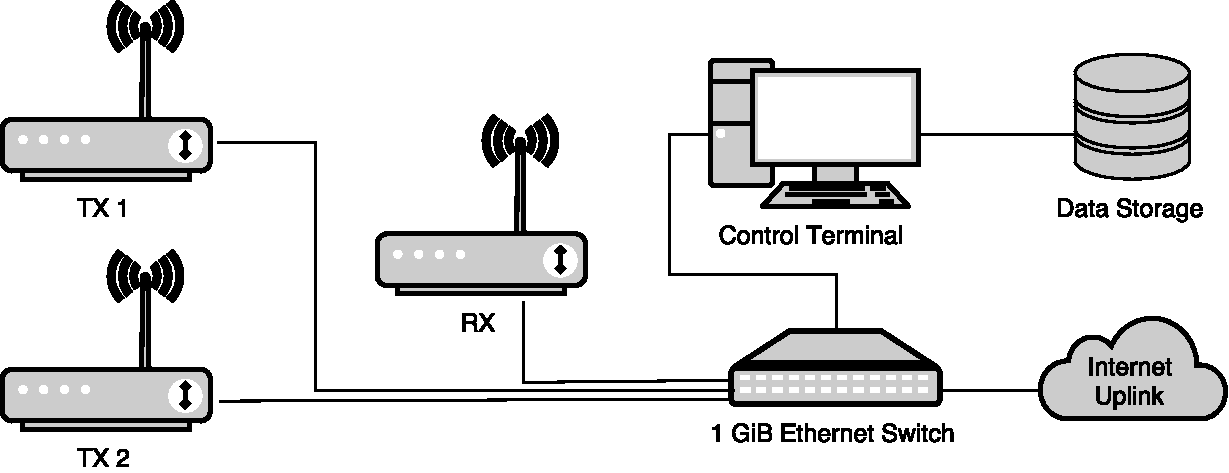
\includegraphics[width=\textwidth]{gfx/images/warp-layout}
	\caption{WARP SDR Experiments Hardware Layout}
	\label{fig:warp-layout}
\end{figure}

The experiments were carried out in a typical office building. This means that there were multiple IEEE 802.11 networks with several dozens of connected clients. I used a standard WLAN channel and no electomagnetic shielding.\\

Since the \gls{WARP} boards use a sampling frequency of 40 MHz, but the Matlab WLAN Systems Toolbox creates time-domain samples with a 20 MHz sampling rate, I used interpolation to adapt frequencies. This is done with the built-in \texttt{interp} Matlab function. Listing \ref{lst:interp} illustrates the process.

\begin{lstlisting}[captionpos=b,caption={Interpolate Sampling Rate},label=lst:interp]
% Interpolate to get from 20 to 40 MHz sampling rate
tx1 = interp(tx1, 2);
\end{lstlisting}

For the real-world experiments, I collided packets with the same scrambler initialization and destination MAC addresses, and used \gls{MCS} 0. This means that in principal everything was the same as for the most basic simulation experiments.

Unfortunately, the sender detection did not work at all with \gls{WARP} \glspl{SDR}. Over quite a long period of experimentation time, sender guesses were not more correct than what would be expected from a random distribution.\\

While trying to find hints on why the technique seemed broken, I wondered if maybe the capture effect as described in section \ref{} affected the received samples in such a way that detection was impossible.

I applied cross-correlation to a \gls{LTF} symbol instead of the MAC addresses and plotted the results. They can be seen in figure \ref{fig:warp_preamble_corr}. The collided frames were aligned with some offset for this experiment.

While one group of spikes is a bit lower than the other, it is still easily possible to detect that there is a collision due to the 4 higher and 2 lower spikes caused by the two \glspl{LTF}. The higher level of noise in the begining of the signal are caused by \gls{AGC} in the receiving \gls{SDR}. Since the MAC addresses are located further into the signal, and only that part is correlated for sender detection, this noise should be no problem.

\begin{figure}[H]
	\centering
	\setlength\figureheight{5cm}
	\setlength\figurewidth{0.9\textwidth}
	% uncomment the following line to recompile the figure when it changes otherwise a cached version is used
	%\tikzset{external/remake next}
	% This file was created by matlab2tikz.
%
%The latest updates can be retrieved from
%  http://www.mathworks.com/matlabcentral/fileexchange/22022-matlab2tikz-matlab2tikz
%where you can also make suggestions and rate matlab2tikz.
%
\begin{tikzpicture}[%
font=\footnotesize
]

\begin{axis}[%
width=0.951\figurewidth,
height=\figureheight,
at={(0\figurewidth,0\figureheight)},
scale only axis,
xmin=0,
xmax=1800,
ymin=0,
ymax=3,
axis background/.style={fill=white},
title style={font=\bfseries},
title={LTF correlation for real-world samples},
axis x line*=bottom,
axis y line*=left,
legend style={legend cell align=left, align=left, draw=white!15!black},
clip mode=individual,transpose legend,legend columns=2,legend style={at={(0,1)},anchor=north west,draw=black,fill=white,legend cell align=left}
]
\addplot [color=blue, line width=1.0pt, mark=*, mark options={solid, blue}]
  table[row sep=crcr]{%
0	0.720931094814423\\
1	1.16568673441402\\
2	1.3141546759545\\
3	0.641645290157508\\
4	0.395108219802532\\
5	1.02254413691229\\
6	1.23346012773391\\
7	1.42940247728357\\
8	1.30855846240446\\
9	0.792541754711272\\
10	0.677926422656566\\
11	0.763008367099554\\
12	0.572326863744454\\
13	0.649448460335741\\
14	0.812836127899684\\
15	0.639897774704796\\
16	0.502144929911757\\
17	0.640000230333206\\
18	0.81890427349694\\
19	1.53125596120855\\
20	1.8355736526179\\
21	1.18894623425786\\
22	0.60757103489733\\
23	0.407157849107528\\
24	0.699168812767027\\
25	1.59107505149703\\
26	1.43988110173639\\
27	1.37478224378645\\
28	2.149245777478\\
29	1.76369670544532\\
30	0.483670341471905\\
31	0.720050971652801\\
32	0.577076089785491\\
33	0.864228058873508\\
34	1.7400151550178\\
35	1.60627196930859\\
36	1.10858033190134\\
37	0.906993644997446\\
38	0.466732145205898\\
39	0.758335526961838\\
40	0.923912129091483\\
41	0.562123267347041\\
42	0.146318849471526\\
43	0.299150577295798\\
44	0.518541495586723\\
45	0.307678574313589\\
46	0.269363873348616\\
47	0.7841954651033\\
48	0.903290445718305\\
49	0.771001575016175\\
50	1.37252584723606\\
51	1.97341433169664\\
52	1.84990733323974\\
53	1.38084133037432\\
54	1.27928436110181\\
55	0.850531224546523\\
56	0.770733316261401\\
57	1.57252407213278\\
58	1.27841331252654\\
59	0.775021234513872\\
60	1.58959359668981\\
61	1.54008487485559\\
62	0.944250193569413\\
63	0.903618738844383\\
64	0.808518293906735\\
65	1.26113739140597\\
66	1.58295659094252\\
67	1.17050995255307\\
68	0.473145617440272\\
69	0.366412679946316\\
70	0.594788181609445\\
71	0.548538264495461\\
72	0.357807390986729\\
73	0.467814304964996\\
74	0.39858933272967\\
75	0.39133352216922\\
76	0.29014892545605\\
77	0.414382894055281\\
78	0.691198625034713\\
79	0.451295808218838\\
80	0.336777310915194\\
81	0.673566047736059\\
82	0.736654379278464\\
83	1.17905398352261\\
84	1.51883016653246\\
85	1.32439126197165\\
86	1.00600801576514\\
87	0.963546970549056\\
88	1.18006580980734\\
89	1.25349188629195\\
90	0.762923878560664\\
91	1.12990732924819\\
92	1.67390574330647\\
93	1.21911492682408\\
94	0.725775917654175\\
95	0.906257359262177\\
96	0.79359366771158\\
97	1.34538942764149\\
98	1.61536202534121\\
99	1.32048539338983\\
100	1.01812234763284\\
101	0.591981636089268\\
102	0.370843752321289\\
103	0.525446350300325\\
104	0.0531063527778062\\
105	0.602782140312682\\
106	0.9925350287863\\
107	0.889246032822645\\
108	0.414779769670687\\
109	0.429045440294952\\
110	0.918347836443727\\
111	0.787004409124193\\
112	0.0640846830193087\\
113	0.70839962170215\\
114	1.03855374671624\\
115	0.772946558469687\\
116	0.475001387401616\\
117	0.696477679643915\\
118	0.812466249307104\\
119	0.868370373915567\\
120	0.77569356256677\\
121	0.520636853334394\\
122	0.817592638653556\\
123	1.20595902508417\\
124	1.07296506081179\\
125	0.698172053895777\\
126	1.01856457142272\\
127	1.10954500520664\\
128	0.791248583502632\\
129	0.948277538125297\\
130	0.962877522329877\\
131	0.511015199610062\\
132	0.316811014975686\\
133	0.243392905032121\\
134	0.247417245739964\\
135	0.60408716366557\\
136	0.515351365618617\\
137	0.140029251031592\\
138	0.281398869611954\\
139	0.479328866858171\\
140	0.492905940122276\\
141	0.467124543000461\\
142	0.430931151562365\\
143	0.254032927394278\\
144	0.393369736537108\\
145	0.610705190118998\\
146	0.599891193561674\\
147	0.534322709031245\\
148	0.506749062094263\\
149	0.606530494360062\\
150	0.786256344223052\\
151	0.842088797648275\\
152	0.717315789990021\\
153	0.396612166978163\\
154	0.590618822960569\\
155	0.661243410011752\\
156	0.494646879338831\\
157	0.528392735902201\\
158	0.664038681511439\\
159	0.635322247949787\\
160	0.746189844141419\\
161	0.796185035737734\\
162	0.444645157646661\\
163	0.105367523231385\\
164	0.462759538553399\\
165	0.528502846102991\\
166	0.447561848084432\\
167	0.272947785051632\\
168	0.161697362821431\\
169	0.21934718394202\\
170	0.161857317123406\\
171	0.126760061054273\\
172	0.104667768489787\\
173	0.245152265595692\\
174	0.383178680584173\\
175	0.401820121385813\\
176	0.384852177380141\\
177	0.364535067975096\\
178	0.297874363959069\\
179	0.405516937768411\\
180	0.585421660014701\\
181	0.617698531786405\\
182	0.546337347184682\\
183	0.533466097046177\\
184	0.623059927555602\\
185	0.603682182501965\\
186	0.3988094949763\\
187	0.200985911686892\\
188	0.36040025909977\\
189	0.588826598028605\\
190	0.682585079801368\\
191	0.679289292813292\\
192	0.761875072505756\\
193	0.698516815309861\\
194	0.39421147625963\\
195	0.276052017302006\\
196	0.328173765579516\\
197	0.352938489363377\\
198	0.49936154530006\\
199	0.478941854678629\\
200	0.316216628578522\\
201	0.284481384532082\\
202	0.305176674189754\\
203	0.24654769175249\\
204	0.113572281764097\\
205	0.202486135424496\\
206	0.28997574217328\\
207	0.208581405848185\\
208	0.108292644688327\\
209	0.169527694743327\\
210	0.297418899441112\\
211	0.429937223568841\\
212	0.43570541297004\\
213	0.4124175737342\\
214	0.471594738112648\\
215	0.405230696692198\\
216	0.406921704076214\\
217	0.575618191362919\\
218	0.48878883605\\
219	0.169130999319071\\
220	0.567054895581535\\
221	0.85262387819276\\
222	0.77816908415513\\
223	0.557048282992595\\
224	0.493846137795923\\
225	0.509416315343237\\
226	0.443475650423118\\
227	0.247407494096242\\
228	0.350565851265824\\
229	0.605479729595615\\
230	0.529929464221523\\
231	0.19690633646066\\
232	0.243364953771876\\
233	0.210329810576645\\
234	0.21937051796833\\
235	0.527037808309991\\
236	0.626557594360931\\
237	0.467382636567737\\
238	0.162633364607986\\
239	0.184995571095381\\
240	0.26246213333078\\
241	0.0821647749139948\\
242	0.270526287960425\\
243	0.437176949343445\\
244	0.302789595703765\\
245	0.171002169950304\\
246	0.316708251796659\\
247	0.276169073916823\\
248	0.332452471436443\\
249	0.469483989661724\\
250	0.385734487612786\\
251	0.200509931930949\\
252	0.25204172112822\\
253	0.504007585976586\\
254	0.701693246140831\\
255	0.824194265991174\\
256	0.886150226418558\\
257	0.839686220654251\\
258	0.65026667423914\\
259	0.389181632780917\\
260	0.395650617968788\\
261	0.616696237425897\\
262	0.718932827668808\\
263	0.647710770975872\\
264	0.550861303398622\\
265	0.450146320767909\\
266	0.412634190553644\\
267	0.579066853708034\\
268	0.597760345697625\\
269	0.426102032379351\\
270	0.337646287985447\\
271	0.328176469575033\\
272	0.259884442540605\\
273	0.106654710453866\\
274	0.208984579514297\\
275	0.348482290942643\\
276	0.299623990902014\\
277	0.185337646753725\\
278	0.248431484437914\\
279	0.319426358645417\\
280	0.2772272175275\\
281	0.266320662016076\\
282	0.302359122889774\\
283	0.1295808165565\\
284	0.256798588657833\\
285	0.618669631925832\\
286	0.747481217358204\\
287	0.668802436681065\\
288	0.521261676168647\\
289	0.387264596851937\\
290	0.421927502752322\\
291	0.412880147967949\\
292	0.44093250357214\\
293	0.740522556061655\\
294	0.84493967584052\\
295	0.70879846409772\\
296	0.527019992968485\\
297	0.446707596894314\\
298	0.922924696516647\\
299	1.33860491392172\\
300	1.16373851032171\\
301	0.550601006176828\\
302	0.457963004040581\\
303	0.583541129603565\\
304	0.37844202335645\\
305	0.148802044337363\\
306	0.0643794430407777\\
307	0.0699834185368895\\
308	0.061950902565579\\
309	0.0019552948287911\\
310	0.0747935165795\\
311	0.192455676578184\\
312	0.241462953288397\\
313	0.192589186111211\\
314	0.239512960969524\\
315	0.105756428246341\\
316	0.278102811389726\\
317	0.597147363484762\\
318	0.60448465931663\\
319	0.464636656167896\\
320	0.43724956929255\\
321	0.403090206001361\\
322	0.457400795038727\\
323	0.482701590105114\\
324	0.570512550744854\\
325	0.670777770100924\\
326	0.526133133681203\\
327	0.438132042371519\\
328	0.558709667575666\\
329	0.526842875064231\\
330	0.547016416661765\\
331	0.686957039296202\\
332	0.619633653152223\\
333	0.446535743665881\\
334	0.401598165478051\\
335	0.26295788991983\\
336	0.140291712994303\\
337	0.205874982385661\\
338	0.169661704066953\\
339	0.0624727817771767\\
340	0.0893189391578162\\
341	0.206600773096695\\
342	0.229952737486357\\
343	0.103883987007097\\
344	0.182407278735709\\
345	0.413230478610313\\
346	0.48156266905976\\
347	0.370049439642338\\
348	0.40538385916249\\
349	0.575515219196783\\
350	0.582529342292222\\
351	0.536169673359967\\
352	0.50223149344944\\
353	0.468877540957649\\
354	0.544389491162411\\
355	0.541534218040889\\
356	0.599045296240793\\
357	0.744769347128761\\
358	0.647465449906921\\
359	0.468725541265581\\
360	0.552110239416768\\
361	0.541555701800614\\
362	0.522590997478641\\
363	0.685577820123613\\
364	0.67601962887479\\
365	0.429600866634372\\
366	0.261877522010782\\
367	0.227408262911671\\
368	0.133497588871437\\
369	0.089945183166874\\
370	0.102587420522226\\
371	0.0804193476926125\\
372	0.0791667341329972\\
373	0.172331402914878\\
374	0.273997943835839\\
375	0.255174555723054\\
376	0.156559063610574\\
377	0.253249409823208\\
378	0.354421169283508\\
379	0.44035592187088\\
380	0.558788816431985\\
381	0.597831387477915\\
382	0.623806910205155\\
383	0.750927920520728\\
384	0.810386708930307\\
385	0.734001927474996\\
386	0.626627199890916\\
387	0.513933611241598\\
388	0.464879776843613\\
389	0.522537413387102\\
390	0.472707109212168\\
391	0.35198434236775\\
392	0.396984895454405\\
393	0.396884367714415\\
394	0.278056664674387\\
395	0.330093375350994\\
396	0.400853525190633\\
397	0.287393979226489\\
398	0.107769990829097\\
399	0.120752691598849\\
400	0.130345260940638\\
401	0.124302926768883\\
402	0.119781298917038\\
403	0.10724548380331\\
404	0.0749766422282917\\
405	0.0696248294056397\\
406	0.0681030770244627\\
407	0.0807744817031463\\
408	0.191314611252934\\
409	0.139263889875701\\
410	0.229041304184165\\
411	0.526275432216956\\
412	0.701293042452557\\
413	0.722321553526931\\
414	0.608695795865329\\
415	0.470250071026404\\
416	0.372382486666876\\
417	0.342238357747492\\
418	0.581727864448338\\
419	0.645478709394455\\
420	0.535502720123082\\
421	0.640355412522363\\
422	0.669522583261143\\
423	0.662384186739298\\
424	0.530603718722175\\
425	0.613766447794406\\
426	1.62962815873112\\
427	2.18742149731996\\
428	1.75063274281811\\
429	0.713207227160355\\
430	0.332529025298972\\
431	0.466168870128803\\
432	0.212629992007919\\
433	0.0696353788421605\\
434	0.0292271723798141\\
435	0.0487973338728497\\
436	0.0378511297748502\\
437	0.145987764444517\\
438	0.163896206279309\\
439	0.135259008653192\\
440	0.107909610136488\\
441	0.0867524219458357\\
442	0.12768496006025\\
443	0.143553785797558\\
444	0.357587974327753\\
445	0.514104735948499\\
446	0.483547763275411\\
447	0.422729230262341\\
448	0.397699201703674\\
449	0.277495362749907\\
450	0.34121589990255\\
451	0.435990378710489\\
452	0.46308636142043\\
453	0.653436524347772\\
454	0.685546696138492\\
455	0.475514977166753\\
456	0.457403743120247\\
457	0.643545047376216\\
458	0.820065664848105\\
459	0.855048760871613\\
460	0.631459686448819\\
461	0.238692606641416\\
462	0.109936427343734\\
463	0.225743573261735\\
464	0.205057250220913\\
465	0.209545612633914\\
466	0.194307456419798\\
467	0.212013010702738\\
468	0.315592792921871\\
469	0.374044718614761\\
470	0.322196908830155\\
471	0.199943557666601\\
472	0.183571035581014\\
473	0.203629935828034\\
474	0.0967061348641033\\
475	0.317954836994668\\
476	0.558435943629889\\
477	0.628958225214659\\
478	0.58599120797271\\
479	0.521177888862574\\
480	0.441692616623721\\
481	0.362237162660365\\
482	0.348123877856604\\
483	0.24667760681855\\
484	0.0927457314340676\\
485	0.390266834901365\\
486	0.506903449647394\\
487	0.329534002725255\\
488	0.231083438639872\\
489	0.321385464652983\\
490	0.301439202980121\\
491	0.423071804787139\\
492	0.510397848551832\\
493	0.441686612223795\\
494	0.306567348541328\\
495	0.229532864078417\\
496	0.212948528430432\\
497	0.344720113604652\\
498	0.751355359009571\\
499	1.19341460357228\\
500	1.32029379390884\\
501	0.982902203486811\\
502	0.457420925332982\\
503	0.448599403332307\\
504	0.509341117371367\\
505	0.268401526425729\\
506	0.0450638880970166\\
507	0.155546304715029\\
508	0.123518368779894\\
509	0.229780171386422\\
510	0.380687471099624\\
511	0.531265332343756\\
512	0.611674281278041\\
513	0.510239718334173\\
514	0.206356913472231\\
515	0.163056622459863\\
516	0.397043288038431\\
517	0.373029910696369\\
518	0.187826502544895\\
519	0.186351304877066\\
520	0.143911842690011\\
521	0.0919027122842002\\
522	0.285106790008328\\
523	0.376514008930879\\
524	0.330948670750887\\
525	0.243736103314185\\
526	0.194453546686479\\
527	0.215527260740158\\
528	0.270914893776744\\
529	0.280952361841279\\
530	0.328851221032298\\
531	0.355120198419307\\
532	0.246621493916162\\
533	0.122421211315998\\
534	0.241784890945979\\
535	0.399879468695546\\
536	0.386981682143234\\
537	0.146802945342198\\
538	0.190101043474684\\
539	0.354635196984993\\
540	0.256362366935009\\
541	0.202145416770583\\
542	0.275975619479487\\
543	0.226249791938257\\
544	0.181515901056431\\
545	0.183981631139009\\
546	0.14700641268006\\
547	0.0767713417808291\\
548	0.353891609790477\\
549	0.396779493948713\\
550	0.065014749739428\\
551	0.471968106924515\\
552	0.4665234658575\\
553	0.699590373039856\\
554	1.64135520528653\\
555	1.91092390697065\\
556	1.20813116917421\\
557	0.125100764508337\\
558	0.492964451692283\\
559	0.345725762430673\\
560	0.119367159623564\\
561	0.243208022465742\\
562	0.106844054970704\\
563	0.441731174060692\\
564	0.515015412294371\\
565	0.304916788848737\\
566	0.123566332112047\\
567	0.11819235961056\\
568	0.0379660573172009\\
569	0.105342995804198\\
570	0.0548198690840899\\
571	0.132003648163404\\
572	0.245283806080487\\
573	0.323736087640489\\
574	0.426908786011443\\
575	0.461868744581769\\
576	0.381357991192025\\
577	0.180615401503067\\
578	0.0422839812668914\\
579	0.0870583734129203\\
580	0.102729756668487\\
581	0.190698642907933\\
582	0.209365093465682\\
583	0.173519112596846\\
584	0.141780768568869\\
585	0.0471237112534095\\
586	0.0839856422532778\\
587	0.0975443658481744\\
588	0.168890661065352\\
589	0.261569354576836\\
590	0.167375007827894\\
591	0.123784536573176\\
592	0.344569095775757\\
593	0.360173966085722\\
594	0.219608993100634\\
595	0.166929239182116\\
596	0.17934005497151\\
597	0.0935966832277601\\
598	0.0822743037972114\\
599	0.174260037661151\\
600	0.204598898824003\\
601	0.10319176931733\\
602	0.199960882689767\\
603	0.460861184832484\\
604	0.538102234209114\\
605	0.385700753282671\\
606	0.168091302189618\\
607	0.170066095147624\\
608	0.150228058831398\\
609	0.173892894895959\\
610	0.32303169823533\\
611	0.294465048718059\\
612	0.150392496197543\\
613	0.357088317376207\\
614	0.534191946235149\\
615	0.465236266689985\\
616	0.229437168196802\\
617	0.1787559957163\\
618	0.0235683872542294\\
619	0.340514543717646\\
620	0.483301905003438\\
621	0.136070481276109\\
622	0.511422722392272\\
623	0.779470773884751\\
624	0.552127012557067\\
625	0.293965169544466\\
626	0.728527067842925\\
627	1.92741364670176\\
628	2.76126966263812\\
629	2.32218416126096\\
630	0.823476352969465\\
631	0.757600741126276\\
632	1.13469399302578\\
633	0.512119633385463\\
634	0.446400493246496\\
635	0.75836182055086\\
636	0.589067160630994\\
637	0.37905794392298\\
638	0.316812474253128\\
639	0.305450964733822\\
640	0.411043581989764\\
641	0.427106762218403\\
642	0.328250113650151\\
643	0.26924910437628\\
644	0.369608682235869\\
645	0.545590263146875\\
646	0.51095126624569\\
647	0.225969068566234\\
648	0.0937504933582185\\
649	0.155691757863386\\
650	0.143563257569863\\
651	0.351751358524464\\
652	0.433949888254632\\
653	0.357377637035286\\
654	0.214611614026436\\
655	0.149150874346242\\
656	0.307133618961262\\
657	0.445991544391623\\
658	0.446780348229075\\
659	0.316092954418524\\
660	0.237936921677401\\
661	0.331447133374475\\
662	0.401124318471257\\
663	0.429152751370368\\
664	0.489548512639156\\
665	0.558465944697459\\
666	0.557289567781402\\
667	0.435843112962036\\
668	0.287024219880359\\
669	0.355205661752089\\
670	0.497515711480277\\
671	0.531266933596987\\
672	0.511681944710538\\
673	0.464540147486314\\
674	0.332596060914124\\
675	0.158226012455663\\
676	0.014064244121227\\
677	0.16322630420039\\
678	0.256088197379928\\
679	0.140405968224649\\
680	0.138933251088646\\
681	0.362448154041183\\
682	0.328641526594172\\
683	0.0768127486016245\\
684	0.384845493789722\\
685	0.482809793757096\\
686	0.275457514423422\\
687	0.0530417323123215\\
688	0.268408350840961\\
689	0.299749000323586\\
690	0.283898391991072\\
691	0.31595235382063\\
692	0.325186823438073\\
693	0.364058648683932\\
694	0.421687748481671\\
695	0.358488699794597\\
696	0.141064270962358\\
697	0.123110445853515\\
698	0.223346033159042\\
699	0.237056305046239\\
700	0.351137018832305\\
701	0.420089415453384\\
702	0.38676276652493\\
703	0.342165439154439\\
704	0.257617649191544\\
705	0.129631691943858\\
706	0.102069193589967\\
707	0.180578295632904\\
708	0.301444002698921\\
709	0.336558240944508\\
710	0.281824011800399\\
711	0.286293675127396\\
712	0.402233019751339\\
713	0.523937042275589\\
714	0.588326894756645\\
715	0.636902666331705\\
716	0.617199255461832\\
717	0.412922613399484\\
718	0.156349702270328\\
719	0.117043838122135\\
720	0.0829060412724096\\
721	0.117524377907638\\
722	0.162973175072084\\
723	0.153400691364329\\
724	0.155761355919494\\
725	0.136505908666391\\
726	0.171157307898558\\
727	0.315735424875619\\
728	0.40461518778541\\
729	0.303507250567475\\
730	0.0483486889728578\\
731	0.260672915757872\\
732	0.4378087280427\\
733	0.377545678447735\\
734	0.249940420286451\\
735	0.230510124707139\\
736	0.0807542714077559\\
737	0.223955075594841\\
738	0.417924833504463\\
739	0.382960190580908\\
740	0.230991749352918\\
741	0.217866072182273\\
742	0.259138390261212\\
743	0.15926043649283\\
744	0.160276929577583\\
745	0.368243891262315\\
746	0.266660499707543\\
747	0.0867255979748171\\
748	0.308207283774522\\
749	0.337854629420402\\
750	0.392685997932947\\
751	0.248407149353968\\
752	0.110689032013529\\
753	0.100710789577973\\
754	0.892288182394515\\
755	2.09382446624789\\
756	2.72470634861384\\
757	2.27675888323154\\
758	1.1048354005623\\
759	0.226444553580792\\
760	0.369864784351082\\
761	0.148496302986251\\
762	0.365909290815374\\
763	0.578604806929237\\
764	0.654476355668374\\
765	0.687499399988648\\
766	0.567210356681008\\
767	0.301658546688265\\
768	0.0861310867565108\\
769	0.14846355624387\\
770	0.0995700847362622\\
771	0.143875236501039\\
772	0.389489306782707\\
773	0.417962803226999\\
774	0.230849392667428\\
775	0.361682033254571\\
776	0.583304032543313\\
777	0.615267969742941\\
778	0.45043856213961\\
779	0.183215266958946\\
780	0.294618630234423\\
781	0.367472403217824\\
782	0.28867754268478\\
783	0.268665809606939\\
784	0.310565815729897\\
785	0.189865358428593\\
786	0.113698506102315\\
787	0.366620280575616\\
788	0.454536407047754\\
789	0.372589715719288\\
790	0.241980359965275\\
791	0.34976453245567\\
792	0.662577186432819\\
793	0.841524117152697\\
794	0.716005275127444\\
795	0.331030214489267\\
796	0.250144896561747\\
797	0.449989176152152\\
798	0.327684151304352\\
799	0.123866547932481\\
800	0.326521572234744\\
801	0.470510345760954\\
802	0.585410715276073\\
803	0.632918141515959\\
804	0.770145897070932\\
805	1.0016042480738\\
806	0.963117036501962\\
807	0.514322799162361\\
808	0.37323405525437\\
809	0.597743450479532\\
810	0.315490613586239\\
811	0.208054317321593\\
812	0.462301152403848\\
813	0.255827124984059\\
814	0.463020198255113\\
815	0.944596262342304\\
816	1.11759538454457\\
817	1.01220163116186\\
818	0.78900310133871\\
819	0.487556736437165\\
820	0.44301664118515\\
821	0.634236253453442\\
822	0.357557033583092\\
823	0.32850876953164\\
824	0.866194518175319\\
825	0.845466292276557\\
826	0.338485526354025\\
827	0.235440966410065\\
828	0.333226140420261\\
829	0.200646713494725\\
830	0.340872647510832\\
831	0.270273983035593\\
832	0.192448921722253\\
833	0.484896293904654\\
834	0.451977294820869\\
835	0.2849984536338\\
836	0.717342889084254\\
837	1.03050679519872\\
838	0.946487938823356\\
839	0.481260957218292\\
840	0.145304001353818\\
841	0.493649897983945\\
842	0.585434107017717\\
843	0.568750458513584\\
844	0.578379026679306\\
845	0.677112466134451\\
846	0.773487569592078\\
847	0.678688970458506\\
848	0.421757035797303\\
849	0.2010576960115\\
850	0.19277736270908\\
851	0.277599395814113\\
852	0.443628705738444\\
853	0.621054613271224\\
854	0.597393241573949\\
855	0.379979473497789\\
856	0.264784173047269\\
857	0.314257544445957\\
858	0.315291996084775\\
859	0.17725450429281\\
860	0.251416215795789\\
861	0.458076562431085\\
862	0.482037570301275\\
863	0.311524892391306\\
864	0.406386224835557\\
865	0.700325161227682\\
866	0.90092444867141\\
867	0.931777201215463\\
868	0.730868391450711\\
869	0.382514810859039\\
870	0.41352761570972\\
871	0.627894590807779\\
872	0.617899435559013\\
873	0.64207227087695\\
874	0.72886369486967\\
875	0.598596620180397\\
876	0.318310803702694\\
877	0.131709128367549\\
878	0.118179883343233\\
879	0.189556078563537\\
880	0.17781323599985\\
881	0.389564363991561\\
882	0.672205993409351\\
883	0.669718091752701\\
884	0.369472221493465\\
885	0.211527861038651\\
886	0.359648591242743\\
887	0.335095273956787\\
888	0.068483572010832\\
889	0.353621066309294\\
890	0.568877644257586\\
891	0.512116123644591\\
892	0.363679148902602\\
893	0.288405450400304\\
894	0.22326926166577\\
895	0.176885819615737\\
896	0.143154711145315\\
897	0.380298239514034\\
898	0.614558038215729\\
899	0.578721040014523\\
900	0.21139161194512\\
901	0.478174607734529\\
902	0.926275928433847\\
903	0.997289257818208\\
904	0.77947958085551\\
905	0.576055322186855\\
906	0.49035681801128\\
907	0.460677476901321\\
908	0.386568329360941\\
909	0.209387809400451\\
910	0.200327469427142\\
911	0.230691513087918\\
912	0.192932952506158\\
913	0.503266993024592\\
914	0.755507328596432\\
915	0.809045996551424\\
916	0.767021286444002\\
917	0.671065960090064\\
918	0.484883129151955\\
919	0.230074327994701\\
920	0.128995454838941\\
921	0.345289479117791\\
922	0.384530814718324\\
923	0.292102302697931\\
924	0.298194920185229\\
925	0.35771921663781\\
926	0.394110421937291\\
927	0.431825529604142\\
928	0.553954180352857\\
929	0.716574681295351\\
930	0.676863649329791\\
931	0.339434413748892\\
932	0.284926107480752\\
933	0.536176706352768\\
934	0.409485156296245\\
935	0.0762554688483868\\
936	0.381893559603867\\
937	0.591039664532489\\
938	0.717101620199821\\
939	0.744777453233646\\
940	0.597789905799106\\
941	0.354750384906439\\
942	0.141721272283775\\
943	0.0911511701068049\\
944	0.324441072364926\\
945	0.461859561931817\\
946	0.511780721756483\\
947	0.444893522509152\\
948	0.234716421721703\\
949	0.186950925756396\\
950	0.298056607842396\\
951	0.405147744830547\\
952	0.615414575875029\\
953	0.770303101705183\\
954	0.661038925155761\\
955	0.239378433920133\\
956	0.365514705120487\\
957	0.67376659181255\\
958	0.547328374349141\\
959	0.305730004524237\\
960	0.503619749928028\\
961	0.585707110598313\\
962	0.459221706332411\\
963	0.294895170063773\\
964	0.488273674110233\\
965	0.745203734028448\\
966	0.64626480370085\\
967	0.264948406022545\\
968	0.361722366213968\\
969	0.486496333188186\\
970	0.295219887811328\\
971	0.129587843218795\\
972	0.285823624471815\\
973	0.451867922940138\\
974	0.575316066695998\\
975	0.509671043852899\\
976	0.417299228166569\\
977	0.496436062428654\\
978	0.403912769597126\\
979	0.404639763167882\\
980	0.695908585816227\\
981	0.650959266534144\\
982	0.246281558474422\\
983	0.305011672241064\\
984	0.441007638268125\\
985	0.259551396929417\\
986	0.165688273042358\\
987	0.241582589764807\\
988	0.371211893805178\\
989	0.546969484095499\\
990	0.424203832364138\\
991	0.0452383346885032\\
992	0.585255029354417\\
993	0.909120952621958\\
994	0.946811307020979\\
995	0.788343965788801\\
996	0.386546193458253\\
997	0.239025539584588\\
998	0.642674117585814\\
999	0.606721730003367\\
1000	0.592404430132469\\
1001	1.03245015558821\\
1002	1.20503527281041\\
1003	0.928624688851519\\
1004	0.498314311077874\\
1005	0.349173572074039\\
1006	0.607183413147065\\
1007	0.763295105733744\\
1008	0.570345455987628\\
1009	0.21093011888463\\
1010	0.215819881142273\\
1011	0.144461284832156\\
1012	0.283619701229973\\
1013	0.560104217293436\\
1014	0.444574345032972\\
1015	0.346305885930186\\
1016	0.794927016549784\\
1017	0.904694076731957\\
1018	0.668544506897595\\
1019	0.528020390528739\\
1020	0.477734566047601\\
1021	0.227119071141285\\
1022	0.0925806252615383\\
1023	0.25067287828687\\
1024	0.283187457148412\\
1025	0.379950655052656\\
1026	0.49112718634571\\
1027	0.484495701019795\\
1028	0.363910694066386\\
1029	0.253655544960424\\
1030	0.349967028147319\\
1031	0.475196603542184\\
1032	0.426949660516203\\
1033	0.169082090744189\\
1034	0.162119757585455\\
1035	0.339376359084902\\
1036	0.259816193941616\\
1037	0.0412933281173994\\
1038	0.185584914987884\\
1039	0.320377974683441\\
1040	0.334370156070599\\
1041	0.33331436860529\\
1042	0.53520542233906\\
1043	0.769969398221327\\
1044	0.854821529024577\\
1045	0.800875856051569\\
1046	0.687423797502815\\
1047	0.545289680196176\\
1048	0.42167654154754\\
1049	0.42841287148455\\
1050	0.457620099842055\\
1051	0.372898849396488\\
1052	0.435698731565404\\
1053	0.522148097710112\\
1054	0.46973975231359\\
1055	0.522808385813571\\
1056	0.598475629155794\\
1057	0.526006123640873\\
1058	0.378789260486091\\
1059	0.140254970361527\\
1060	0.309262419596818\\
1061	0.559509266463221\\
1062	0.444685801464865\\
1063	0.180903613123284\\
1064	0.375480830790108\\
1065	0.486759948062772\\
1066	0.528990062898542\\
1067	0.690590499514008\\
1068	0.825094891624801\\
1069	0.734675746313926\\
1070	0.477332325473237\\
1071	0.217382606934343\\
1072	0.135171217567511\\
1073	0.279336680480251\\
1074	0.445957842365257\\
1075	0.460734973751249\\
1076	0.34985151711341\\
1077	0.303178153572367\\
1078	0.311144788015777\\
1079	0.262159179469428\\
1080	0.228502472370588\\
1081	0.226380896291226\\
1082	0.281467948209267\\
1083	0.557433535699452\\
1084	0.67183231063932\\
1085	0.375671449583628\\
1086	0.365741672063115\\
1087	0.766083911967129\\
1088	0.720087427482685\\
1089	0.380953990653822\\
1090	0.106769914684017\\
1091	0.241901772157984\\
1092	0.537688374778057\\
1093	0.650568738555171\\
1094	0.536890085191081\\
1095	0.455555163306814\\
1096	0.58621486718669\\
1097	0.707034653989684\\
1098	0.65530032417563\\
1099	0.489747111200401\\
1100	0.338151122593478\\
1101	0.251979898003424\\
1102	0.135855279159459\\
1103	0.215803588864905\\
1104	0.650360464681284\\
1105	0.882057484209142\\
1106	0.70019725987026\\
1107	0.353104412148447\\
1108	0.256587715738428\\
1109	0.237288037810344\\
1110	0.393964746137633\\
1111	0.476217075736521\\
1112	0.318033905928838\\
1113	0.443879095276938\\
1114	0.644794411414292\\
1115	0.501330978557401\\
1116	0.34218826846042\\
1117	0.59975282667751\\
1118	0.639671175083582\\
1119	0.529440269571555\\
1120	0.442703961150953\\
1121	0.265571595743326\\
1122	0.0689799097070581\\
1123	0.0295184044071393\\
1124	0.302260497346136\\
1125	0.723842675428941\\
1126	1.03098294540808\\
1127	1.01794838350118\\
1128	0.69036817228119\\
1129	0.356142128195849\\
1130	0.251905649516953\\
1131	0.0457731851139892\\
1132	0.254567692822892\\
1133	0.3688442612567\\
1134	0.236323872144101\\
1135	0.0679040881632075\\
1136	0.125461525072873\\
1137	0.469010299655276\\
1138	0.765268684112713\\
1139	0.605334258081494\\
1140	0.110805941330764\\
1141	0.65413473645282\\
1142	0.775929830163297\\
1143	0.33783528857876\\
1144	0.499959376291521\\
1145	0.991085767405238\\
1146	1.04473372207031\\
1147	0.862493951239157\\
1148	0.828939012039119\\
1149	0.700123345347914\\
1150	0.328977766369524\\
1151	0.472657154435168\\
1152	0.773172140703431\\
1153	0.697150003185472\\
1154	0.378670664484028\\
1155	0.221105301360738\\
1156	0.383486203379865\\
1157	0.545016184823472\\
1158	0.511244904370802\\
1159	0.39227687059048\\
1160	0.460807570279434\\
1161	0.439523697281284\\
1162	0.291494522656188\\
1163	0.383684232703596\\
1164	0.519634197540048\\
1165	0.61932903215293\\
1166	0.761265289935176\\
1167	0.803016168115657\\
1168	0.647991605263647\\
1169	0.602866526857985\\
1170	0.773911131826815\\
1171	0.736470442948859\\
1172	0.572068499897697\\
1173	0.58688891169514\\
1174	0.53193265149407\\
1175	0.295734220097046\\
1176	0.145461313482281\\
1177	0.0991807112175916\\
1178	0.224273205654516\\
1179	0.478316398035087\\
1180	0.559783638091041\\
1181	0.356184834686581\\
1182	0.0453274277599695\\
1183	0.343521703226387\\
1184	0.270827194586928\\
1185	0.162427060387293\\
1186	0.534254838013541\\
1187	0.640866133262533\\
1188	0.462657131574164\\
1189	0.172418666693398\\
1190	0.224854468024476\\
1191	0.418669374328701\\
1192	0.488612052152037\\
1193	0.588817912376539\\
1194	0.77360374248751\\
1195	0.812018551301868\\
1196	0.658352789595154\\
1197	0.390596231400963\\
1198	0.23827148136614\\
1199	0.404827095768551\\
1200	0.458691478726506\\
1201	0.300815515886928\\
1202	0.137324499370226\\
1203	0.192771691782227\\
1204	0.197961361748826\\
1205	0.262875959586602\\
1206	0.513629515085065\\
1207	0.658929408589692\\
1208	0.62628468586425\\
1209	0.401864753268883\\
1210	0.418855399059409\\
1211	0.929971335270184\\
1212	1.09304835565284\\
1213	0.647408845547438\\
1214	0.146694813090288\\
1215	0.603089680390987\\
1216	0.5841488546429\\
1217	0.333378120106976\\
1218	0.34985671638862\\
1219	0.299355121876421\\
1220	0.407219086419217\\
1221	0.605232209341661\\
1222	0.592956925612315\\
1223	0.532856920497668\\
1224	0.59106296842982\\
1225	0.61984232372637\\
1226	0.520755847761676\\
1227	0.338911192911197\\
1228	0.214643970178203\\
1229	0.332313998414965\\
1230	0.557451650066823\\
1231	0.714965617649123\\
1232	0.693508699799119\\
1233	0.497820549883622\\
1234	0.229763244220124\\
1235	0.116698895862632\\
1236	0.143712139309626\\
1237	0.0626835357143963\\
1238	0.171615001161818\\
1239	0.224652994070805\\
1240	0.157032787671615\\
1241	0.223628704389018\\
1242	0.268512572569072\\
1243	0.109916879148358\\
1244	0.183170719689723\\
1245	0.202630051511414\\
1246	0.271150301827152\\
1247	0.550903828648659\\
1248	0.556520755988829\\
1249	0.184023952889716\\
1250	0.325121751144312\\
1251	0.525034679801723\\
1252	0.446567720983772\\
1253	0.43986823241786\\
1254	0.360307583004613\\
1255	0.291917748925662\\
1256	0.526778102163278\\
1257	0.473602111066009\\
1258	0.150203972358194\\
1259	0.498038640805559\\
1260	0.719681661404805\\
1261	0.530355745447569\\
1262	0.132779501378234\\
1263	0.547625044845395\\
1264	0.87262052544942\\
1265	0.845448945970716\\
1266	0.570558607969083\\
1267	0.30716266192415\\
1268	0.224379441038601\\
1269	0.256888346326299\\
1270	0.281433419924608\\
1271	0.327782452239766\\
1272	0.233830663408589\\
1273	0.259773287580726\\
1274	0.708583714735372\\
1275	0.951285282807045\\
1276	0.881864177328423\\
1277	0.70344340414887\\
1278	0.486100309189704\\
1279	0.428583390388548\\
1280	0.664360069128585\\
1281	0.607372433909361\\
1282	0.430946045052881\\
1283	0.546728475566623\\
1284	0.393762968204706\\
1285	0.231078260967565\\
1286	0.573098363495476\\
1287	0.434542295305657\\
1288	0.352371377285696\\
1289	0.747537064510239\\
1290	0.610621102269335\\
1291	0.0747920167346156\\
1292	0.475832030844646\\
1293	0.410130751725635\\
1294	0.16547996611665\\
1295	0.578930763884711\\
1296	0.651049540373431\\
1297	0.531029451179755\\
1298	0.432366339840194\\
1299	0.130185243981183\\
1300	0.31726363500407\\
1301	0.480090960913724\\
1302	0.226926168568983\\
1303	0.36601594436566\\
1304	0.630906682990481\\
1305	0.492293528475987\\
1306	0.160454502598636\\
1307	0.256593594491305\\
1308	0.160818566535714\\
1309	0.242753384299684\\
1310	0.437269131423912\\
1311	0.421284028374232\\
1312	0.37973116848521\\
1313	0.226902995070559\\
1314	0.152660218731496\\
1315	0.503422345959693\\
1316	0.577248098355658\\
1317	0.640724226041516\\
1318	0.796339264758414\\
1319	0.57352494397008\\
1320	0.130246140716947\\
1321	0.741283678916919\\
1322	0.859313882981998\\
1323	0.389706361576307\\
1324	0.340196487812669\\
1325	0.770704054540422\\
1326	0.837866279533662\\
1327	0.935400134899361\\
1328	1.03905743039519\\
1329	0.795925771530005\\
1330	0.468032723565019\\
1331	0.539873684392969\\
1332	0.605687510681739\\
1333	0.500576545780843\\
1334	0.346263654443717\\
1335	0.259816805008787\\
1336	0.664034475052776\\
1337	0.968595214884648\\
1338	0.8824804880205\\
1339	0.533724640621101\\
1340	0.227783428249371\\
1341	0.20249437737224\\
1342	0.293130549517616\\
1343	0.159046050217638\\
1344	0.36377413233226\\
1345	0.69752114031682\\
1346	0.652099903024062\\
1347	0.307334395570351\\
1348	0.223854651493835\\
1349	0.30168208871521\\
1350	0.207828604479985\\
1351	0.343799698865816\\
1352	0.533610839914502\\
1353	0.70556680256432\\
1354	0.863192795087905\\
1355	0.831737747556242\\
1356	0.631907029087104\\
1357	0.5137763528493\\
1358	0.585196099286018\\
1359	0.613702054817861\\
1360	0.602936153783279\\
1361	0.567399964914442\\
1362	0.589320445954468\\
1363	0.764057654163899\\
1364	0.803958595123603\\
1365	0.579186512191239\\
1366	0.25996479291888\\
1367	0.122498625348993\\
1368	0.155464229200524\\
1369	0.33165550761421\\
1370	0.565820310402731\\
1371	0.67158584363341\\
1372	0.52862799172766\\
1373	0.18009410056957\\
1374	0.170094383848948\\
1375	0.358153528480492\\
1376	0.416830070706143\\
1377	0.388002202757937\\
1378	0.333692190705088\\
1379	0.577876406791921\\
1380	0.781234780537293\\
1381	0.590130036925739\\
1382	0.215144485880523\\
1383	0.377997633866649\\
1384	0.334165715505774\\
1385	0.347712491684665\\
1386	0.605494306550604\\
1387	0.558779162658729\\
1388	0.275030291429447\\
1389	0.438048885110263\\
1390	0.615210082588837\\
1391	0.470376200099858\\
1392	0.075376165123468\\
1393	0.317479368063406\\
1394	0.460959272202355\\
1395	0.289061590065403\\
1396	0.0965547109431708\\
1397	0.429068038699018\\
1398	0.684747053717749\\
1399	0.802095111877916\\
1400	0.660591680312876\\
1401	0.284518302401025\\
1402	0.112793071141255\\
1403	0.252839929596487\\
1404	0.153441295287371\\
1405	0.0936919140959101\\
1406	0.164971311747485\\
1407	0.155397031489008\\
1408	0.115285135714112\\
1409	0.0340923476570214\\
1410	0.0799583256368405\\
1411	0.164281044903229\\
1412	0.217778476425612\\
1413	0.236353930910212\\
1414	0.237218514936038\\
1415	0.430002868388864\\
1416	0.637022472259674\\
1417	0.57019516048719\\
1418	0.224922262017431\\
1419	0.291774544804939\\
1420	0.506593593206139\\
1421	0.440514998058237\\
1422	0.279382172276462\\
1423	0.211445482168005\\
1424	0.293144781968962\\
1425	0.384622427109352\\
1426	0.238848945352705\\
1427	0.147317755794344\\
1428	0.409681653271499\\
1429	0.328744534530124\\
1430	0.307495569650739\\
1431	0.577393295878819\\
1432	0.542850189786511\\
1433	0.365796175090139\\
1434	0.513229149573472\\
1435	0.534608164456783\\
1436	0.495918766262856\\
1437	0.668277855201852\\
1438	0.744073976097762\\
1439	0.764702737189493\\
1440	0.934586837577323\\
1441	1.03812218248735\\
1442	0.836191214565965\\
1443	0.464258566959064\\
1444	0.169535901094871\\
1445	0.113992130113522\\
1446	0.254808324581197\\
1447	0.49980735527322\\
1448	0.748036409192327\\
1449	0.851605365317003\\
1450	0.762001275749619\\
1451	0.602776861356764\\
1452	0.417481710675782\\
1453	0.321747881724357\\
1454	0.424646541446106\\
1455	0.379908396369887\\
1456	0.161342177031815\\
1457	0.19801631102434\\
1458	0.299799029235775\\
1459	0.262251885965337\\
1460	0.0887279057633941\\
1461	0.108515857436239\\
1462	0.173849196024466\\
1463	0.157468459263039\\
1464	0.337071186146531\\
1465	0.536626375916972\\
1466	0.553205772905676\\
1467	0.347342421089263\\
1468	0.19724716152145\\
1469	0.494271554916131\\
1470	0.698499306279125\\
1471	0.691930691183403\\
1472	0.606375629859606\\
1473	0.707518250906747\\
1474	0.824616213688261\\
1475	0.793500224582173\\
1476	0.729366637033635\\
1477	0.664611738597242\\
1478	0.52370230940254\\
1479	0.333514585471706\\
1480	0.238534216177588\\
1481	0.306084159235254\\
1482	0.424997771970866\\
1483	0.505791990487111\\
1484	0.750215597554343\\
1485	0.961646143370971\\
1486	0.783346529075394\\
1487	0.371102482964568\\
1488	0.265176950414104\\
1489	0.194714110789823\\
1490	0.382257204936566\\
1491	0.498624847956222\\
1492	0.304282106676666\\
1493	0.0294748766772345\\
1494	0.11657125649192\\
1495	0.212232346605573\\
1496	0.210276142287185\\
1497	0.164668224241788\\
1498	0.656823222786021\\
1499	1.09572279941734\\
1500	1.23271820206479\\
1501	1.02382180752791\\
1502	0.657754359733899\\
1503	0.356484330115183\\
1504	0.15590374047752\\
1505	0.187342635823333\\
1506	0.241514321563142\\
1507	0.396893267721729\\
1508	0.604339451345821\\
1509	0.655254102938723\\
1510	0.542009433502955\\
1511	0.469100638897761\\
1512	0.453113492760237\\
1513	0.314607514309541\\
1514	0.137343416317913\\
1515	0.16826299140548\\
1516	0.181742377470477\\
1517	0.182797846910563\\
1518	0.308689656918434\\
1519	0.589123323601346\\
1520	0.835313388164985\\
1521	0.751629003459079\\
1522	0.425765689694949\\
1523	0.547828969070655\\
1524	0.603914655637977\\
1525	0.15056488390933\\
1526	0.679036644064575\\
1527	1.14609056122336\\
1528	1.01815139649352\\
1529	0.528707778915703\\
1530	0.456121770035782\\
1531	0.637418301682629\\
1532	0.604897211403683\\
1533	0.494209605889778\\
1534	0.392914525483137\\
1535	0.291254055925102\\
1536	0.18767357227049\\
1537	0.0207076900994457\\
1538	0.238374902563699\\
1539	0.474789185025303\\
1540	0.583533472171029\\
1541	0.404006993570605\\
1542	0.203710792284998\\
1543	0.605502417188802\\
1544	0.704593915047504\\
1545	0.444880526841348\\
1546	0.279093387169363\\
1547	0.292639014473523\\
1548	0.215049338488645\\
1549	0.270326950837429\\
1550	0.244801524994023\\
1551	0.181510477580052\\
1552	0.224869918924013\\
1553	0.271706678252936\\
1554	0.274144619033362\\
1555	0.17580625686758\\
1556	0.242694444525501\\
1557	0.258397950526723\\
1558	0.0956599162969102\\
1559	0.290222185569757\\
1560	0.351433561121964\\
1561	0.300394374565569\\
1562	0.479265168397394\\
1563	0.649328211190724\\
1564	0.634663383590059\\
1565	0.547333661679593\\
1566	0.494284355040153\\
1567	0.494290642689591\\
1568	0.565686580797289\\
1569	0.560437415132723\\
1570	0.424243327881649\\
1571	0.345848926254892\\
1572	0.438231643285417\\
1573	0.615049252673882\\
1574	0.701390423424249\\
1575	0.622700803693321\\
1576	0.674977636619207\\
1577	0.953149809404131\\
1578	1.0393326994093\\
1579	0.849832443716062\\
1580	0.502794951175903\\
1581	0.211727202939577\\
1582	0.32342952961564\\
1583	0.506574826803359\\
1584	0.627119819372067\\
1585	0.642723340756867\\
1586	0.641888180423328\\
1587	0.756943166760529\\
1588	0.84814669773893\\
1589	0.68161657518207\\
1590	0.32363378714536\\
1591	0.32192449704191\\
1592	0.501449757455932\\
1593	0.435855020329214\\
1594	0.34711203952262\\
1595	0.443056135385426\\
1596	0.444965646273248\\
1597	0.300563784592226\\
1598	0.0764264434798999\\
1599	0.181695904004665\\
1600	0.334579393179548\\
1601	0.319044405760889\\
1602	0.445031691929692\\
1603	0.629429890692383\\
1604	0.493733679381599\\
1605	0.152155005505426\\
1606	0.0759928109827516\\
1607	0.0914807713113918\\
1608	0.295623186276377\\
1609	0.380502247066614\\
1610	0.278497491019325\\
1611	0.41292227879425\\
1612	0.655171716295165\\
1613	0.775315486282599\\
1614	0.696294952709069\\
1615	0.433711974700216\\
1616	0.0862681763965909\\
1617	0.376883810257876\\
1618	0.673774013762568\\
1619	0.733483198095749\\
1620	0.551110686876951\\
1621	0.334866439383021\\
1622	0.335490053758092\\
1623	0.282014204821392\\
1624	0.204297074105571\\
1625	0.292157906209206\\
1626	0.359948300288946\\
1627	0.331901332884775\\
1628	0.255948939125909\\
1629	0.255151019654955\\
1630	0.266720614039642\\
1631	0.168961479149183\\
1632	0.179284972580033\\
1633	0.382252994018345\\
1634	0.427137736627872\\
1635	0.319231601711931\\
1636	0.585044016277411\\
1637	0.841536394691967\\
1638	0.754912513932417\\
1639	0.415081467743279\\
1640	0.199399019259145\\
1641	0.392068873063899\\
1642	0.611797588998442\\
1643	0.680657938972765\\
1644	0.563426494184934\\
1645	0.787709302015365\\
1646	1.20594359538766\\
1647	1.29837578605631\\
1648	0.998701783130613\\
1649	0.715611903207284\\
1650	0.588676241494111\\
1651	0.279792462229601\\
1652	0.528165602933636\\
1653	0.800935453727805\\
1654	0.714922357792839\\
1655	0.627488151798378\\
1656	0.663887348016648\\
1657	0.497836241079376\\
1658	0.327088688908173\\
1659	0.347322188750708\\
1660	0.238329328289809\\
1661	0.0712864695448951\\
1662	0.379588755149812\\
1663	0.483105518939034\\
1664	0.303578630991329\\
1665	0.206145496176095\\
1666	0.401980103987141\\
1667	0.287190020018585\\
1668	0.105419643485365\\
1669	0.466999461841536\\
1670	0.540043817356454\\
1671	0.400177355704686\\
1672	0.359828155374772\\
1673	0.433206439170569\\
1674	0.54323097556504\\
1675	0.60751248011818\\
1676	0.590795541352951\\
1677	0.546809246778224\\
1678	0.5169894031549\\
1679	0.413795733187278\\
1680	0.166765951294089\\
1681	0.148878372014209\\
1682	0.224984937243948\\
1683	0.188444103082586\\
1684	0.409156725507385\\
1685	0.511658960979729\\
1686	0.532633195126255\\
1687	0.719299166955618\\
1688	0.830567382328121\\
1689	0.677732142356846\\
1690	0.338113815824965\\
1691	0.00864796147419466\\
1692	0.178513036165022\\
1693	0.264815414319966\\
1694	0.431297379954816\\
1695	0.537636733031649\\
1696	0.528537937856241\\
1697	0.484294479402469\\
1698	0.429906035094518\\
1699	0.420193200253821\\
1700	0.489625022718731\\
1701	0.410818966893969\\
1702	0.144009561097052\\
1703	0.409040468083817\\
1704	0.514610200631623\\
1705	0.380100524103092\\
1706	0.632816129130505\\
1707	0.865802787218027\\
1708	0.658942182772927\\
1709	0.17332413720837\\
1710	0.430888467321637\\
1711	0.620386895143715\\
1712	0.731575804065528\\
1713	0.783684272381219\\
1714	0.602088489365523\\
1715	0.249224913746784\\
1716	0.188812519764418\\
1717	0.328894448080919\\
1718	0.347852006080635\\
1719	0.325963981818339\\
1720	0.363001156143509\\
1721	0.4444449199134\\
1722	0.380202400768175\\
1723	0.070289721244262\\
1724	0.441836250245204\\
1725	0.643757758342175\\
1726	0.46803402986558\\
1727	0.166031957412227\\
1728	0.45395808451906\\
1729	0.702141426244159\\
1730	0.703784407490947\\
1731	0.495285724817464\\
1732	0.229362470829893\\
1733	0.18018516447027\\
1734	0.318944384864367\\
1735	0.317927445283448\\
1736	0.46054154051984\\
1737	0.702589027811511\\
1738	0.683943442583302\\
1739	0.373775816084005\\
1740	0.169722520634252\\
1741	0.338315240238975\\
1742	0.144333870543602\\
1743	0.440384307761278\\
1744	0.814420358699666\\
1745	0.718483647597573\\
1746	0.32268731585597\\
1747	0.359864963641841\\
1748	0.207848986539807\\
1749	0.345323283707884\\
1750	0.718899145383002\\
1751	0.602093901217059\\
1752	0.14298844148785\\
1753	0.220527145071217\\
1754	0.32640146345477\\
1755	0.521787416108978\\
1756	0.651294591329915\\
1757	0.587014598532468\\
1758	0.526052230201919\\
1759	0.573603752973317\\
1760	0.680416753269935\\
1761	0.732169462452854\\
1762	0.680776645788326\\
1763	0.627892728867725\\
1764	0.503636633987628\\
1765	0.211073442047971\\
1766	0.106748562463938\\
1767	0.2519104558373\\
1768	0.249547372212585\\
1769	0.308564718556851\\
1770	0.371665881955158\\
1771	0.215738701813582\\
1772	0.129847039022412\\
1773	0.318679907180183\\
1774	0.192558895691456\\
1775	0.219297589936507\\
1776	0.586573491221457\\
1777	0.666228111212966\\
1778	0.523869784327977\\
1779	0.374741248077429\\
1780	0.243525301902685\\
1781	0.3114380934455\\
1782	0.409703985961431\\
1783	0.521656342436072\\
1784	0.777787192321129\\
1785	0.894272496841148\\
1786	0.726396159372864\\
1787	0.424452791460504\\
1788	0.303573113318997\\
1789	0.414723850765126\\
1790	0.498864057096193\\
1791	0.482815293125504\\
1792	0.294890405512635\\
1793	0.248904065020524\\
1794	0.575710431415076\\
1795	0.636076427713717\\
1796	0.442446388957629\\
1797	0.443854020601148\\
1798	0.523214396256606\\
1799	0.425124359277182\\
1800	0.201744379056123\\
1801	0.232109527902345\\
1802	0.414974456144079\\
1803	0.474769246837259\\
1804	0.481632610438582\\
1805	0.377076821374018\\
1806	0.32677729387552\\
1807	0.391087274691477\\
1808	0.159493085451673\\
1809	0.337192868726371\\
1810	0.633087865580532\\
1811	0.561651065938799\\
1812	0.321369064292441\\
1813	0.15161088652274\\
1814	0.206574082764142\\
1815	0.447062249551755\\
1816	0.610215060409397\\
1817	0.648215897876746\\
1818	0.674025408997679\\
1819	0.729340456211708\\
1820	0.698660790594277\\
1821	0.541160782392076\\
1822	0.466185921581845\\
1823	0.550623649997345\\
1824	0.606986123731155\\
1825	0.516171265549133\\
1826	0.345226442558457\\
1827	0.248191179778469\\
1828	0.0892266998795086\\
1829	0.433909341962317\\
1830	0.754318129309783\\
1831	0.664431641323019\\
1832	0.329225829178854\\
1833	0.655409375235393\\
1834	0.729642090549517\\
1835	0.382752268731833\\
1836	0.656446849303817\\
1837	0.967394567844947\\
1838	0.900884884647638\\
1839	0.815477882057038\\
1840	0.792280007705258\\
1841	0.715799514332808\\
1842	0.683125675196396\\
1843	0.691752660208801\\
1844	0.572318506740686\\
1845	0.268882608027113\\
1846	0.20265260884146\\
1847	0.537353796860442\\
1848	0.675935613686201\\
1849	0.547771642363726\\
1850	0.143182021207272\\
1851	0.402145168062323\\
1852	0.690501532912754\\
1853	0.576053182123254\\
1854	0.284082162876035\\
1855	0.334521188018458\\
1856	0.142370838658672\\
1857	0.42363827390215\\
1858	0.854454957975878\\
1859	0.798287821589539\\
1860	0.624514351774396\\
1861	0.906409172067576\\
1862	1.00226550734445\\
1863	0.749606569771726\\
1864	0.50371736167051\\
1865	0.465389713935086\\
1866	0.532793809914006\\
1867	0.543473276857849\\
1868	0.469212063806816\\
1869	0.459104715646875\\
1870	0.440760921931601\\
1871	0.293198970709976\\
1872	0.133154622443362\\
1873	0.0872376709119251\\
1874	0.18130100745058\\
1875	0.249879819440566\\
1876	0.241986487424363\\
1877	0.259862040075429\\
1878	0.315833362768093\\
1879	0.324173875089168\\
1880	0.354927558284102\\
1881	0.332242780649641\\
1882	0.152313127279675\\
1883	0.087915981429259\\
1884	0.249263379638627\\
1885	0.272092125327508\\
1886	0.177073618935148\\
1887	0.0550400321095974\\
1888	0.0460076618309449\\
1889	0.163245750685168\\
1890	0.372961458958888\\
1891	0.417133398283721\\
1892	0.127048350914136\\
1893	0.344229035256574\\
1894	0.579277843719862\\
1895	0.391657446652552\\
1896	0.312962950975955\\
1897	0.580727781734763\\
1898	0.696142656221254\\
1899	0.798543596928025\\
1900	0.69980281023454\\
1901	0.284395466561834\\
1902	0.155209643675847\\
1903	0.189784908146297\\
1904	0.155176894581428\\
1905	0.441540453544867\\
1906	0.479876166554192\\
1907	0.304162023366081\\
1908	0.119011862119111\\
1909	0.0927537325081903\\
1910	0.130351550387097\\
1911	0.26216560964769\\
1912	0.409592820460911\\
1913	0.467693987626284\\
1914	0.380450436670171\\
1915	0.194299386629225\\
1916	0.259266058939441\\
1917	0.519984680916362\\
1918	0.604559131626093\\
1919	0.546050205094811\\
1920	0.6952774313474\\
1921	0.873111280853375\\
1922	0.801624105620298\\
1923	0.558907204646593\\
1924	0.217492902352898\\
1925	0.216626005739245\\
1926	0.536596589788816\\
1927	0.57157918963123\\
1928	0.545541628660225\\
1929	0.727889258677625\\
1930	0.836831375687247\\
1931	0.736799568615183\\
1932	0.591253411639962\\
1933	0.515553043125483\\
1934	0.468085569712334\\
1935	0.380608388740755\\
1936	0.239330342330169\\
1937	0.0993733391149632\\
1938	0.0709798726861005\\
1939	0.118839633150212\\
1940	0.169667368973162\\
1941	0.253631075213541\\
1942	0.291523198188598\\
1943	0.239451785393032\\
1944	0.172223080925841\\
1945	0.184309541688092\\
1946	0.255257386620725\\
1947	0.283402023958552\\
1948	0.316967899961962\\
1949	0.431514965653381\\
1950	0.564777164686913\\
1951	0.645180459793204\\
1952	0.637086985634417\\
1953	0.596256196278814\\
1954	0.605843435490969\\
1955	0.517635707686791\\
1956	0.294497922785423\\
1957	0.324262135264488\\
1958	0.408356308004844\\
1959	0.311590712120873\\
1960	0.393828413782572\\
1961	0.595912287640783\\
1962	0.668337842726345\\
1963	0.569063345909705\\
1964	0.384995559298892\\
1965	0.362748762668723\\
1966	0.376502307727034\\
1967	0.234134661314317\\
1968	0.126500134195505\\
1969	0.122826363133129\\
1970	0.111021296507554\\
1971	0.424401588387867\\
1972	0.527360455151492\\
1973	0.361004883662187\\
1974	0.212211727095242\\
1975	0.0993463450662114\\
1976	0.114767680587397\\
1977	0.18422711770695\\
1978	0.133071734823673\\
1979	0.500937504909985\\
1980	0.716611086135447\\
1981	0.603465594208894\\
1982	0.438592064201311\\
1983	0.385298656650456\\
1984	0.243723054779003\\
1985	0.244652261155884\\
1986	0.323480210615731\\
1987	0.212023710735374\\
1988	0.100990112849386\\
1989	0.460548149877939\\
1990	0.815147656390236\\
1991	1.05013948358504\\
1992	1.01448011845534\\
1993	0.682555541522697\\
1994	0.332111623332332\\
1995	0.338791186015819\\
1996	0.420806010476221\\
1997	0.476704336753123\\
1998	0.592357690576171\\
1999	0.704638587096014\\
2000	0.786202402541532\\
2001	0.756256052819903\\
2002	0.496562074509383\\
2003	0.131823377279541\\
2004	0.460403618072595\\
2005	0.66209804889265\\
2006	0.628445639809716\\
2007	0.609028936395521\\
2008	0.611478350901021\\
2009	0.509588377660989\\
2010	0.425546723387229\\
2011	0.377750026508615\\
2012	0.204281141944634\\
2013	0.101838359872192\\
2014	0.232136031336214\\
2015	0.182678272847518\\
2016	0.212508026160534\\
2017	0.331237474514543\\
2018	0.626238762958434\\
2019	0.862505803179862\\
2020	0.705570924169914\\
2021	0.234263582486387\\
2022	0.394989160463975\\
2023	0.576784963713645\\
2024	0.479135457555867\\
2025	0.304267367215268\\
2026	0.372912427980991\\
2027	0.752047804647977\\
2028	0.922444426393113\\
2029	0.685711955801617\\
2030	0.24562570012253\\
2031	0.0952149664980541\\
2032	0.29783468679509\\
2033	0.590454246447768\\
2034	0.713372745693316\\
2035	0.504037630331791\\
2036	0.232730949214758\\
2037	0.684905091770096\\
2038	0.983854994181434\\
2039	0.86612959554855\\
2040	0.552548626945925\\
2041	0.424085925989828\\
2042	0.342987607124723\\
2043	0.182277422292634\\
2044	0.263378332513842\\
2045	0.37339705784727\\
2046	0.39770390543536\\
2047	0.440903110517684\\
2048	0.432184697190136\\
2049	0.336929834621324\\
2050	0.153111949290317\\
2051	0.190154141735944\\
2052	0.488422625853265\\
2053	0.556308175341276\\
2054	0.454345965546173\\
2055	0.406025672573679\\
2056	0.277748980682957\\
2057	0.408016409257264\\
2058	0.672665700553558\\
2059	0.562657891573062\\
2060	0.165844927950249\\
2061	0.226230569495436\\
2062	0.381397103453215\\
2063	0.398357992112354\\
2064	0.348898053708721\\
2065	0.199209160623001\\
2066	0.149630487114522\\
2067	0.341238910873374\\
2068	0.439452639540974\\
2069	0.399455626740179\\
2070	0.364638146776064\\
2071	0.375433326516681\\
2072	0.316324732909768\\
2073	0.265462106513435\\
2074	0.40761072948684\\
2075	0.713412675452743\\
2076	0.872117135048252\\
2077	0.717198158472163\\
2078	0.573382077593219\\
2079	0.613824661400865\\
2080	0.463221315333943\\
2081	0.442760404335731\\
2082	0.656192158553778\\
2083	0.623269309932706\\
2084	0.314941893441745\\
2085	0.162276369665946\\
2086	0.347879821108773\\
2087	0.282177184246495\\
2088	0.151866910445077\\
2089	0.357461649860898\\
2090	0.696883964809186\\
2091	0.886512919331963\\
2092	0.752750695351503\\
2093	0.491751122268583\\
2094	0.375795575762789\\
2095	0.458583713601791\\
2096	0.626104700899833\\
2097	0.727104233572031\\
2098	0.700328622723721\\
2099	0.409465824542444\\
2100	0.342842033804764\\
2101	0.592318540671119\\
2102	0.41689207144557\\
2103	0.0948201377883429\\
2104	0.256871081727152\\
2105	0.0839211495914077\\
2106	0.236237257586215\\
2107	0.341970629691095\\
2108	0.183504208715006\\
2109	0.0615411121344424\\
2110	0.165289517183725\\
2111	0.136991944143538\\
2112	0.261850156241755\\
2113	0.439909953129805\\
2114	0.459837714317488\\
2115	0.280641864561617\\
2116	0.170410102926545\\
2117	0.405101635719437\\
2118	0.550822821523067\\
2119	0.510905048074835\\
2120	0.431140425310934\\
2121	0.469912582577482\\
2122	0.484404352670057\\
2123	0.397221213792665\\
2124	0.279638857507429\\
2125	0.293147832613153\\
2126	0.51318644236339\\
2127	0.789088411273616\\
2128	0.884472133177166\\
2129	0.757441280666994\\
2130	0.691697249170816\\
2131	0.769563388777948\\
2132	0.683504030759611\\
2133	0.476427582186031\\
2134	0.312775925542627\\
2135	0.322812468917375\\
2136	0.577117132394391\\
2137	0.671538354385498\\
2138	0.489016931595291\\
2139	0.315200645831363\\
2140	0.387282847015285\\
2141	0.386429320476764\\
2142	0.332136871545368\\
2143	0.241778395573182\\
2144	0.0755755275510679\\
2145	0.0473642939032983\\
2146	0.0980371660973691\\
2147	0.385651706018573\\
2148	0.504877666086254\\
2149	0.254855139333829\\
2150	0.253230266969263\\
2151	0.684287815295081\\
2152	0.822128912714925\\
2153	0.718821037164729\\
2154	0.466820253114424\\
2155	0.292583254554298\\
2156	0.521763955613788\\
2157	0.426447336667859\\
2158	0.103171173430472\\
2159	0.664606740922989\\
2160	0.762278560468122\\
2161	0.331364277219764\\
2162	0.462562328348095\\
2163	0.98835193895674\\
2164	1.11739484260639\\
2165	0.761358335848239\\
2166	0.157350133462438\\
2167	0.698617428207171\\
2168	0.93085849188666\\
2169	0.57458248944939\\
2170	0.062453830728176\\
2171	0.448974416161392\\
2172	0.365671542830458\\
2173	0.029594396929891\\
2174	0.138721512423533\\
2175	0.104263988273922\\
2176	0.363726463591261\\
2177	0.414214849521665\\
2178	0.218934352958625\\
2179	0.148655814597516\\
2180	0.307933234319595\\
2181	0.503958929032767\\
2182	0.621255468444863\\
2183	0.69683199149538\\
2184	0.732238881754616\\
2185	0.578049869989625\\
2186	0.319971612082135\\
2187	0.170393381136788\\
2188	0.252443376317474\\
2189	0.48514872189032\\
2190	0.657541219644766\\
2191	0.709313026065473\\
2192	0.670444089442109\\
2193	0.549566064174743\\
2194	0.354133796100334\\
2195	0.471601253955824\\
2196	0.707496768408721\\
2197	0.592365252078036\\
2198	0.205355538437627\\
2199	0.731703701783086\\
2200	1.11635931769367\\
2201	0.988475843326152\\
2202	0.478535623024466\\
2203	0.128111634252745\\
2204	0.297524454627772\\
2205	0.184052240951073\\
2206	0.050848051022857\\
2207	0.119540752401502\\
2208	0.137575648537866\\
2209	0.292470628245326\\
2210	0.395019720744952\\
2211	0.463078803358207\\
2212	0.650424902602407\\
2213	0.667772375160705\\
2214	0.326919052720565\\
2215	0.529017587620689\\
2216	0.767627821710124\\
2217	0.442416480470324\\
2218	0.310860369860339\\
2219	0.634400147979762\\
2220	0.431683285960708\\
2221	0.209885228398693\\
2222	0.282419784085626\\
2223	0.178053368746103\\
2224	0.298432114371034\\
2225	0.196947199536588\\
2226	0.607294369372543\\
2227	1.03948406290625\\
2228	1.04167748766783\\
2229	0.753231426440755\\
2230	0.402776324740174\\
2231	0.120285138695053\\
2232	0.234787859904334\\
2233	0.182372451872512\\
2234	0.356417302926723\\
2235	0.681481359156523\\
2236	0.695977308712279\\
2237	0.420887547490549\\
2238	0.0583259141512472\\
2239	0.313672772835691\\
2240	0.525302308890079\\
2241	0.484475268221283\\
2242	0.205212607084277\\
2243	0.102807867411926\\
2244	0.14986812951168\\
2245	0.0962270755835339\\
2246	0.307867811228832\\
2247	0.433291835866172\\
2248	0.501266829629842\\
2249	0.597903651802687\\
2250	0.622495874163556\\
2251	0.52283115192181\\
2252	0.439408825472825\\
2253	0.332961300681463\\
2254	0.170666368186098\\
2255	0.0934043663339444\\
2256	0.193689850270776\\
2257	0.531177759928281\\
2258	0.730642725062058\\
2259	0.661768121629161\\
2260	0.487934493874988\\
2261	0.323114665329564\\
2262	0.172680376478545\\
2263	0.365692864951645\\
2264	0.578719345323358\\
2265	0.665871986035861\\
2266	0.518791254583368\\
2267	0.163598494237292\\
2268	0.162437735697073\\
2269	0.225776200805259\\
2270	0.205101055111663\\
2271	0.241734602756543\\
2272	0.298523905106407\\
2273	0.454493222611064\\
2274	0.47043210528253\\
2275	0.3096070714294\\
2276	0.270696962518333\\
2277	0.262267719574812\\
2278	0.16317763018702\\
2279	0.117267226002107\\
2280	0.16944622336406\\
2281	0.378276923197142\\
2282	0.596510806442644\\
2283	0.722277600329865\\
2284	0.64104611149981\\
2285	0.319495949926115\\
2286	0.115836592216267\\
2287	0.253443882547611\\
2288	0.0807630124622878\\
2289	0.386102719568089\\
2290	0.651239411911451\\
2291	0.609181966840279\\
2292	0.444442502668448\\
2293	0.25604725884956\\
2294	0.194166067503929\\
2295	0.583484330338836\\
2296	0.665240307249094\\
2297	0.298240699109718\\
2298	0.385019270705891\\
2299	0.759038538743566\\
2300	0.681986405117584\\
2301	0.293060724931916\\
2302	0.159925783085217\\
2303	0.283380687229277\\
2304	0.51285349308703\\
2305	0.760497215174024\\
2306	0.689090841198422\\
2307	0.411640619072026\\
2308	0.332164061654763\\
2309	0.399723564452948\\
2310	0.467647959629338\\
2311	0.433314509287037\\
2312	0.39303268032868\\
2313	0.699265340997665\\
2314	0.988035104719019\\
2315	0.941426558618909\\
2316	0.573903445689738\\
2317	0.23496267406257\\
2318	0.426303262734387\\
2319	0.539376508845157\\
2320	0.458220010789885\\
2321	0.37302277998908\\
2322	0.416623011979994\\
2323	0.492234018049178\\
2324	0.54281279922741\\
2325	0.479898055718308\\
2326	0.404894211981506\\
2327	0.403139830149409\\
2328	0.326558591890118\\
2329	0.238406008424837\\
2330	0.0784024849615242\\
2331	0.337691253946841\\
2332	0.747027741188508\\
2333	0.848282226500438\\
2334	0.580955685934426\\
2335	0.214878329858553\\
2336	0.0226082810669926\\
2337	0.271824906894174\\
2338	0.658599259668353\\
2339	0.832200677930883\\
2340	0.616849507799825\\
2341	0.192161376680798\\
2342	0.380864237511746\\
2343	0.408768560969854\\
2344	0.121309477477796\\
2345	0.357233459892025\\
2346	0.575072275100789\\
2347	0.467072523045284\\
2348	0.2471292941859\\
2349	0.388191398798884\\
2350	0.38655299882563\\
2351	0.188557570834072\\
2352	0.095488776767105\\
2353	0.0564991837206079\\
2354	0.275113113645942\\
2355	0.385895940714511\\
2356	0.459548876941554\\
2357	0.589761680643968\\
2358	0.507052353648047\\
2359	0.197533454394597\\
2360	0.242865250306375\\
2361	0.226482174031624\\
2362	0.099390531389258\\
2363	0.440448939913211\\
2364	0.552545915978546\\
2365	0.432891550853693\\
2366	0.249394037601182\\
2367	0.0820959293159977\\
2368	0.130224369377083\\
2369	0.1998902260494\\
2370	0.313534276066218\\
2371	0.69554627705728\\
2372	0.970096804525628\\
2373	0.826650863009387\\
2374	0.292878291105766\\
2375	0.333951251561526\\
2376	0.647785063924078\\
2377	0.505560729828527\\
2378	0.260216901704878\\
2379	0.623250918537651\\
2380	0.687092492467244\\
2381	0.318560140750519\\
2382	0.336646622481062\\
2383	0.817582619470432\\
2384	1.09072654830709\\
2385	1.12131320123625\\
2386	0.966235550993818\\
2387	0.691671705193055\\
2388	0.348127636124951\\
2389	0.0524708160505785\\
2390	0.110249629840964\\
2391	0.0659114589994684\\
2392	0.184104759541748\\
2393	0.272912772276616\\
2394	0.31495306205772\\
2395	0.519520412159035\\
2396	0.604798019725406\\
2397	0.410123819455841\\
2398	0.126889487752279\\
2399	0.236473162106588\\
2400	0.366080652950078\\
2401	0.369696904915389\\
2402	0.291808411898205\\
2403	0.227644677970896\\
2404	0.192018538894076\\
2405	0.107115641809094\\
2406	0.0988545513996014\\
2407	0.211998645807942\\
2408	0.336127762397374\\
2409	0.664166188940645\\
2410	0.883372250873197\\
2411	0.630437089235707\\
2412	0.345332247794017\\
2413	0.902700239776331\\
2414	1.07923334420027\\
2415	0.680516922552722\\
2416	0.397870140882259\\
2417	0.791287820668918\\
2418	0.768139562661279\\
2419	0.371497036162821\\
2420	0.368875529067402\\
2421	0.56499292309332\\
2422	0.629640932911192\\
2423	0.734424962463665\\
2424	0.739393275269529\\
2425	0.537304288935762\\
2426	0.316172260500193\\
2427	0.315672260381073\\
2428	0.375219228712145\\
2429	0.502920647514665\\
2430	0.605308144819928\\
2431	0.583639437847615\\
2432	0.414909660969024\\
2433	0.121749759775156\\
2434	0.201878352447949\\
2435	0.373096767206004\\
2436	0.383172105725202\\
2437	0.387475110686276\\
2438	0.417177181295638\\
2439	0.481453471950417\\
2440	0.561015021098289\\
2441	0.517791057592086\\
2442	0.411551782655617\\
2443	0.423151798210766\\
2444	0.493856870730523\\
2445	0.557083804698006\\
2446	0.665308490078401\\
2447	0.816002676905285\\
2448	0.865953192593414\\
2449	0.743418563750632\\
2450	0.568171574352606\\
2451	0.394375782862998\\
2452	0.170008500504822\\
2453	0.306213135265175\\
2454	0.432293399316723\\
2455	0.403401712739727\\
2456	0.334151893760392\\
2457	0.194316755662899\\
2458	0.113552200323938\\
2459	0.333603361534355\\
2460	0.337782567218056\\
2461	0.38425432943479\\
2462	0.697508176251924\\
2463	0.878463655474624\\
2464	0.849348559096258\\
2465	0.761827863660482\\
2466	0.770222872610293\\
2467	0.805673965052126\\
2468	0.720479639718878\\
2469	0.516797210521448\\
2470	0.309850046942156\\
2471	0.270494065658949\\
2472	0.248406187918424\\
2473	0.122816790824152\\
2474	0.238803042916012\\
2475	0.244373768213053\\
2476	0.122071714380395\\
2477	0.395988814970336\\
2478	0.507910095918447\\
2479	0.431889803422749\\
2480	0.560495236119031\\
2481	0.724319958506055\\
2482	0.548931372843372\\
2483	0.152128399029537\\
2484	0.351097112765379\\
2485	0.452487010879978\\
2486	0.388721221600152\\
2487	0.604879483693088\\
2488	0.684675015679223\\
2489	0.357252809191404\\
2490	0.218984426214483\\
2491	0.510290667970156\\
2492	0.419818487541163\\
2493	0.125697533273625\\
2494	0.422545608806378\\
2495	0.561544498752838\\
2496	0.3446779248682\\
2497	0.169792397022498\\
2498	0.51288113363929\\
2499	0.418709333812445\\
2500	0.192834917418304\\
2501	0.62259458653702\\
2502	0.63440902345212\\
2503	0.250468722600444\\
2504	0.187840317611922\\
2505	0.171628203306892\\
2506	0.318935787075608\\
2507	0.562777927095789\\
2508	0.648690216664694\\
2509	0.670618521339283\\
2510	0.683241273363139\\
2511	0.666353589379494\\
2512	0.521988992218709\\
2513	0.160816736405685\\
2514	0.351924237207107\\
2515	0.673287218568801\\
2516	0.712987123386769\\
2517	0.538410848144212\\
2518	0.298837660328634\\
2519	0.191844228308135\\
2520	0.311385160359598\\
2521	0.485842555687534\\
2522	0.547861872405787\\
2523	0.435939607253063\\
2524	0.290739171773254\\
2525	0.214004953371685\\
2526	0.135160136873069\\
2527	0.180700922755539\\
2528	0.211678761107281\\
2529	0.340017328705734\\
2530	0.828272892174902\\
2531	1.12221076460034\\
2532	0.894377270243091\\
2533	0.451105766864189\\
2534	0.683652833269965\\
2535	0.755543343208853\\
2536	0.360592077547043\\
2537	0.312399270234679\\
2538	0.663811346931144\\
2539	0.683060385789572\\
2540	0.476102207851042\\
2541	0.344195385279901\\
2542	0.485906783068071\\
2543	0.599507674302956\\
2544	0.47829499747364\\
2545	0.378868379888887\\
2546	0.55599961753804\\
2547	0.574884826277062\\
2548	0.355305398697653\\
2549	0.0553431736529224\\
2550	0.183520029121514\\
2551	0.170885729618703\\
2552	0.204727907781408\\
2553	0.521280915555281\\
2554	0.659360199933752\\
2555	0.474241580341751\\
2556	0.409935260936763\\
2557	0.57670501565337\\
2558	0.492060628646494\\
2559	0.36104649753203\\
2560	0.467277055127596\\
2561	0.53568810861621\\
2562	0.532188077797692\\
2563	0.611887873453718\\
2564	0.751840343520059\\
2565	0.782423615907806\\
2566	0.787886150030728\\
2567	0.798875618818168\\
2568	0.599547186751193\\
2569	0.346547529034041\\
2570	0.392833588330027\\
2571	0.371545838516638\\
2572	0.33042668012592\\
2573	0.376482151247394\\
2574	0.326254500670693\\
2575	0.154553082577117\\
2576	0.175409790085204\\
2577	0.414374557476191\\
2578	0.425169635144266\\
2579	0.2384548901923\\
2580	0.302883836508541\\
2581	0.258062855905528\\
2582	0.0688460134669603\\
2583	0.376914888830578\\
2584	0.407222257958267\\
2585	0.185179204884616\\
2586	0.125907688987891\\
2587	0.162074141855665\\
2588	0.445835614663616\\
2589	0.733252500862176\\
2590	0.757253801816232\\
2591	0.611052762506087\\
2592	0.49569111812248\\
2593	0.502527698115421\\
2594	0.682575543766505\\
2595	0.720503370922768\\
2596	0.594911914495004\\
2597	0.735336495379729\\
2598	0.934988819573801\\
2599	0.858645894631095\\
2600	0.545666403168359\\
2601	0.106041426812709\\
2602	0.385226353419871\\
2603	0.775567690556598\\
2604	0.953013227341693\\
2605	0.797435489488455\\
2606	0.444127674679184\\
2607	0.400441362606865\\
2608	0.451004799828556\\
2609	0.553960093038017\\
2610	0.806973401673537\\
2611	0.741596596123361\\
2612	0.274666966383233\\
2613	0.296717036776252\\
2614	0.619002580275588\\
2615	0.644234691579102\\
2616	0.480110713106261\\
2617	0.246377955919503\\
2618	0.0683525752982615\\
2619	0.368472476455402\\
2620	0.46098879869468\\
2621	0.2777847462838\\
2622	0.28366808210918\\
2623	0.453078340245773\\
2624	0.433732234178137\\
2625	0.506655445350639\\
2626	0.526407726712679\\
2627	0.305646286961482\\
2628	0.0381902323852245\\
2629	0.100498103776612\\
2630	0.0522309420787739\\
2631	0.314033731016869\\
2632	0.530637316799885\\
2633	0.531304658787448\\
2634	0.293474850418173\\
2635	0.0437967243774548\\
2636	0.0685759149619274\\
2637	0.373398188974961\\
2638	0.635981779650688\\
2639	0.530152456764023\\
2640	0.326806121608259\\
2641	0.705457624000179\\
2642	0.840525757832819\\
2643	0.630881149796973\\
2644	0.58076969156397\\
2645	0.60646726569733\\
2646	0.423041501247986\\
2647	0.461032931389744\\
2648	0.512333711495498\\
2649	0.385158808101022\\
2650	0.156385575279112\\
2651	0.239257315727519\\
2652	0.662085314942432\\
2653	0.74848356233487\\
2654	0.319258252290664\\
2655	0.385127187977205\\
2656	0.86105524113669\\
2657	0.980533731981672\\
2658	0.900802832255687\\
2659	0.819684329772105\\
2660	0.724804645637223\\
2661	0.57842243864649\\
2662	0.487438767004113\\
2663	0.438075223419736\\
2664	0.179660127849226\\
2665	0.2752434331927\\
2666	0.594248198399598\\
2667	0.650031510435683\\
2668	0.497914032149186\\
2669	0.396569042746096\\
2670	0.418333683778863\\
2671	0.526732038113499\\
2672	0.687449461652653\\
2673	0.683014080953689\\
2674	0.486508465574287\\
2675	0.261629687080514\\
2676	0.190393360874163\\
2677	0.275272573765048\\
2678	0.387376056348064\\
2679	0.379916498305273\\
2680	0.238474995380166\\
2681	0.0976448626022452\\
2682	0.173500846942502\\
2683	0.226983018980136\\
2684	0.248886002387093\\
2685	0.289954499995025\\
2686	0.309002442785036\\
2687	0.315943498022671\\
2688	0.320539887078342\\
2689	0.241502686067227\\
2690	0.340151956017924\\
2691	0.696528142061882\\
2692	0.837023465677118\\
2693	0.612157648175777\\
2694	0.332106199611008\\
2695	0.492919623866374\\
2696	0.60479366357409\\
2697	0.430334793240443\\
2698	0.277260353369746\\
2699	0.633460094580185\\
2700	0.815582688669703\\
2701	0.62214547845975\\
2702	0.17339349821434\\
2703	0.279116174127969\\
2704	0.534642528849369\\
2705	0.621473547225715\\
2706	0.564404717471551\\
2707	0.456130723852707\\
2708	0.353425692766235\\
2709	0.36221043676556\\
2710	0.579116836164626\\
2711	0.597465703042163\\
2712	0.253296859672558\\
2713	0.422839542069578\\
2714	0.779012982230475\\
2715	0.708066642192159\\
2716	0.368354797378901\\
2717	0.156296734473523\\
2718	0.149633141157318\\
2719	0.570213311503524\\
2720	0.922925798761838\\
2721	0.812529263806461\\
2722	0.252681226225587\\
2723	0.3573004218989\\
2724	0.530479218777974\\
2725	0.253041589100612\\
2726	0.516262001330654\\
2727	0.797021906416936\\
2728	0.708978937395754\\
2729	0.477894711355259\\
2730	0.430230524913688\\
2731	0.451328961593164\\
2732	0.418030494766025\\
2733	0.397779965782937\\
2734	0.401475445465863\\
2735	0.363674414385087\\
2736	0.345976191143251\\
2737	0.326896893448495\\
2738	0.254113995515989\\
2739	0.250438842241948\\
2740	0.346340611807522\\
2741	0.356068433323898\\
2742	0.310840742878802\\
2743	0.332250226177788\\
2744	0.292090963911894\\
2745	0.258675086533339\\
2746	0.280779822406104\\
2747	0.298118975566392\\
2748	0.336631395057401\\
2749	0.360594010847083\\
2750	0.314414546506857\\
2751	0.21660852958448\\
2752	0.38384868598016\\
2753	0.655727246885472\\
2754	0.715238638585038\\
2755	0.55545028378814\\
2756	0.372169904487277\\
2757	0.354248902673036\\
2758	0.441846801230407\\
2759	0.537519238010552\\
2760	0.580982054397361\\
2761	0.522336454592111\\
2762	0.451342741626802\\
2763	0.507707328826896\\
2764	0.428981167463387\\
2765	0.215552196750038\\
2766	0.348106667365461\\
2767	0.540682961389417\\
2768	0.587304202197182\\
2769	0.530464545603214\\
2770	0.560728457355743\\
2771	0.602409824112075\\
2772	0.498721648394185\\
2773	0.33480424181748\\
2774	0.474343206933372\\
2775	0.699301483781716\\
2776	0.746404306760598\\
2777	0.633391180575406\\
2778	0.42151326799198\\
2779	0.156089782397325\\
2780	0.33307525499435\\
2781	0.600743982349584\\
2782	0.65896697367475\\
2783	0.506798631429925\\
2784	0.256895178778491\\
2785	0.116296024664021\\
2786	0.12970219095603\\
2787	0.311769105953759\\
2788	0.483080353030837\\
2789	0.444101023455624\\
2790	0.187403371531068\\
2791	0.240663381783499\\
2792	0.448927946780187\\
2793	0.444261205113396\\
2794	0.290179015425789\\
2795	0.181586839897948\\
2796	0.26284935677442\\
2797	0.239214104451046\\
2798	0.0696289245102543\\
2799	0.131157546962834\\
2800	0.229771413898352\\
2801	0.670330927555257\\
2802	1.19256187669762\\
2803	1.28264138678125\\
2804	0.933810642800727\\
2805	0.751122698267988\\
2806	0.648615863363029\\
2807	0.264795715538412\\
2808	0.52006294875539\\
2809	0.611919630362198\\
2810	0.260453412169309\\
2811	0.344012311398092\\
2812	0.492265440915722\\
2813	0.4768219740966\\
2814	0.469383205521252\\
2815	0.305531686862305\\
2816	0.0524515221576862\\
2817	0.297505876113823\\
2818	0.241807516256212\\
2819	0.0980210517303245\\
2820	0.387689126467692\\
2821	0.325218776167045\\
2822	0.0894888123822346\\
2823	0.408765089214237\\
2824	0.526383202701153\\
2825	0.581676335996294\\
2826	0.558341409989072\\
2827	0.282178026090038\\
2828	0.281688181438658\\
2829	0.456137799845025\\
2830	0.273114186479839\\
2831	0.0761851601868473\\
2832	0.24949233335317\\
2833	0.12976420086205\\
2834	0.155947958090168\\
2835	0.208055682730807\\
2836	0.116272768930604\\
2837	0.292909161168547\\
2838	0.265747601699596\\
2839	0.359351360565508\\
2840	0.591766718738769\\
2841	0.452800145237731\\
2842	0.22905521124639\\
2843	0.466426496073556\\
2844	0.359610427024282\\
2845	0.423663141231086\\
2846	0.864208439994591\\
2847	0.957587662970971\\
2848	0.657114749571923\\
2849	0.315075249287783\\
2850	0.297898827335598\\
2851	0.169796107472986\\
2852	0.0965456411912914\\
2853	0.240610978693463\\
2854	0.166943183894961\\
2855	0.066275208442539\\
2856	0.178257905147472\\
2857	0.20815071723224\\
2858	0.249412806966923\\
2859	0.296211451763708\\
2860	0.277507252207846\\
2861	0.108326387131583\\
2862	0.310264508077565\\
2863	0.59413611618801\\
2864	0.58557806747698\\
2865	0.307604588754809\\
2866	0.22115680502879\\
2867	0.432563430702944\\
2868	0.556505291105714\\
2869	0.792226863395745\\
2870	1.01461055235772\\
2871	0.954135388551596\\
2872	0.5566830698251\\
2873	0.114411546590803\\
2874	0.366508523270216\\
2875	0.496298070276572\\
2876	0.437444349213079\\
2877	0.262510228472639\\
2878	0.203040195929731\\
2879	0.320668989298008\\
2880	0.264109939674988\\
2881	0.195004330463072\\
2882	0.571080236427599\\
2883	0.753777541539555\\
2884	0.589007908795908\\
2885	0.334953501116691\\
2886	0.297129898061457\\
2887	0.206953093931149\\
2888	0.267501735858025\\
2889	0.457763044937252\\
2890	0.496817598029632\\
2891	0.418161353902106\\
2892	0.298714618249832\\
2893	0.19163755082604\\
2894	0.223882665285297\\
2895	0.266247989674296\\
2896	0.367576624098085\\
2897	0.63932156278976\\
2898	0.84993018376426\\
2899	0.859536093942835\\
2900	0.667788771677902\\
2901	0.396304733913131\\
2902	0.196831652500682\\
2903	0.0550782970937651\\
2904	0.291099363330379\\
2905	0.689733636638862\\
2906	0.921323659690369\\
2907	0.757424478566389\\
2908	0.3387211918822\\
2909	0.198872237340901\\
2910	0.177587564974206\\
2911	0.212409044581962\\
2912	0.340899024066134\\
2913	0.227924840134843\\
2914	0.373505106174537\\
2915	0.619180990811718\\
2916	0.496286922307965\\
2917	0.18274063043134\\
2918	0.325132982200334\\
2919	0.341292579609184\\
2920	0.129470304118648\\
2921	0.267093876392548\\
2922	0.421754342855786\\
2923	0.340396052587629\\
2924	0.129866907112207\\
2925	0.350607042469633\\
2926	0.694287975583796\\
2927	1.00175861006277\\
2928	1.10223701606333\\
2929	0.861516791889041\\
2930	0.381574001963019\\
2931	0.384732924232797\\
2932	0.617214347287528\\
2933	0.569778395128849\\
2934	0.52711614462541\\
2935	0.678188105946963\\
2936	0.660106318351845\\
2937	0.376841331971459\\
2938	0.10427871540024\\
2939	0.0733825647106722\\
2940	0.175035459973223\\
2941	0.19401079734211\\
2942	0.355146900964947\\
2943	0.712820226608551\\
2944	0.838174899778083\\
2945	0.619494047498235\\
2946	0.303120239397868\\
2947	0.149308681776949\\
2948	0.0243991047679793\\
2949	0.180085499759422\\
2950	0.271498214584984\\
2951	0.313853247172306\\
2952	0.319548437122617\\
2953	0.323558680469762\\
2954	0.344492399183112\\
2955	0.270503071164872\\
2956	0.401149398292405\\
2957	0.557023540019568\\
2958	0.551389418748485\\
2959	0.476849146236668\\
2960	0.286010126319955\\
2961	0.102930097044064\\
2962	0.324571319751667\\
2963	0.192899548226134\\
2964	0.36287745150451\\
2965	0.805807317645421\\
2966	0.873295132833967\\
2967	0.55723363928397\\
2968	0.202336414822764\\
2969	0.387464302566498\\
2970	0.537101466626018\\
2971	0.518753232661152\\
2972	0.473549436934839\\
2973	0.332089270094607\\
2974	0.0620998640567947\\
2975	0.444774499452775\\
2976	0.659008969713915\\
2977	0.56426400051541\\
2978	0.259146086125496\\
2979	0.142677608087048\\
2980	0.39801406819677\\
2981	0.614835418795059\\
2982	0.700859296157391\\
2983	0.498076524037185\\
2984	0.213498315489178\\
2985	0.463609109651608\\
2986	0.472884944454715\\
2987	0.275157898799295\\
2988	0.312890885916419\\
2989	0.331437125710095\\
2990	0.308685770263008\\
2991	0.329184756365327\\
2992	0.268861801964936\\
2993	0.320307230331213\\
2994	0.415991934497969\\
2995	0.363766916706111\\
2996	0.249452588671153\\
2997	0.290640171135724\\
2998	0.259815978450723\\
2999	0.240276182124714\\
3000	0.50255178964098\\
3001	0.508313899260333\\
3002	0.164718508571872\\
3003	0.522915590160503\\
3004	0.771752522248988\\
3005	0.56254376888211\\
3006	0.414375044181577\\
3007	0.58530936428231\\
3008	0.525934775603493\\
3009	0.517571607829532\\
3010	0.584267414300266\\
3011	0.423843963608353\\
3012	0.214031241076034\\
3013	0.210909721066265\\
3014	0.10039017259611\\
3015	0.114559134585482\\
3016	0.293564006433962\\
3017	0.387689754176915\\
3018	0.415893236958748\\
3019	0.364075658135544\\
3020	0.188468549569863\\
3021	0.263997097986603\\
3022	0.364662535765155\\
3023	0.178353129179622\\
3024	0.161894283137004\\
3025	0.356891832104402\\
3026	0.295359235681265\\
3027	0.186123543332393\\
3028	0.190235082999813\\
3029	0.111074955555478\\
3030	0.181061604237197\\
3031	0.290839329203146\\
3032	0.29209563681503\\
3033	0.172197136019273\\
3034	0.0701765228018253\\
3035	0.174331032138581\\
3036	0.193987705340803\\
3037	0.261793267648201\\
3038	0.298778464888592\\
3039	0.207972519068955\\
3040	0.224420026212278\\
3041	0.292880680914289\\
3042	0.284644136052941\\
3043	0.272414235829225\\
3044	0.172093235982088\\
3045	0.211518872086928\\
3046	0.2398352474982\\
3047	0.0570453323149805\\
3048	0.145282404323055\\
3049	0.143314229452618\\
3050	0.0713122194523107\\
3051	0.0939078707898774\\
3052	0.046759848563673\\
3053	0.213594543908243\\
3054	0.252189321696122\\
3055	0.151646905920037\\
3056	0.159099973049887\\
3057	0.198092297794487\\
3058	0.15071311848097\\
3059	0.0647484669779673\\
3060	0.0713274503295508\\
3061	0.137765791177349\\
3062	0.0986943169385271\\
3063	0.0445669715821388\\
3064	0.0631381521904067\\
3065	0.019282669215936\\
3066	0.101984618885181\\
3067	0.140609074396725\\
3068	0.123823841199595\\
3069	0.136033038507269\\
3070	0.140307233154853\\
3071	0.096087459489906\\
3072	0.112631658587905\\
3073	0.126818978206194\\
3074	0.0301694064531703\\
3075	0.0941102422948428\\
3076	0.122705156700126\\
3077	0.09373565132262\\
3078	0.0842835712084249\\
3079	0.0539243133658129\\
};
\addlegendentry{abs(xcorr(.,.))}

\end{axis}
\end{tikzpicture}%
	\caption{Preamble Correlation in WARP Experiment}
	\label{fig:warp_preamble_corr}
\end{figure}

The results of the preamble correlation are promising and burdernsome at the same time. While they show that indeed a collision of two frames is captured by the receiving \gls{SDR}, and that cross-correlation in the time-domain can in fact tell apart both \glspl{LTF}, they also suggest that there is no fundamental implementation error in the code, but rather that MAC address detection in the form of the presented technique does not work with real-world channel effects.
